\documentclass[../main.tex]{subfiles}

\begin{document}
	
\chapter{Architectural differences in \textit{Cis}\hyp{}regulatory modules between constitutive and variable genes}
\label{chapter1}
%read https://journals.plos.org/plosone/article?id=10.1371/journal.pone.0212678 very relevant
%add poitns from this to intro: https://academic.oup.com/gbe/article/7/4/1002/531003

%point about GC content in plants: https://journals.plos.org/plosone/article?id=10.1371/journal.pone.0212678. They also found that 1. Broadly expressed genes are less compact in nature and 2. Promoters of broadly expressed genes are stable in plants.
%expression level is highly influenced by no. of tissues a gene is expressd in (expression breadth) when expression data is pooled from EST libraries.

%The tissue specificity index τ estimates both qualitative variations (i.e. presence/absence) and quantitative variations of expression level among tissues, which has been suggested to be more representative than expression breadth and expression level for the expression complexity of a gene (Yanai et al. 2005).https://link.springer.com/article/10.1007%2Fs10709-013-9730-9
%evolution:  The resulting data show that PSGs have higher protein evolutionary rates, lower synonymous substitution rates, shorter gene length, fewer exons, higher functional specificity, lower expression level, higher tissue‐specific expression and stronger codon bias than NSGs. https://onlinelibrary.wiley.com/doi/full/10.1111/tpj.13541

% Larger multiple-copy gene families exhibit both lower expression levels and breadth than genes in single-copy gene families17. In addition, tissue-specific expression was more often observed among genes in multiple-copy gene families than genes in single-copy gene families17.https://www.nature.com/articles/s41598-017-13981-1#Sec9
%"wide range of abiotic and biotic treatments, the application of plant hormones and other chemical treatments performed, and were designed to enable comparative studies by using the same technology platform and reference condition."" We define the term “breadth of response” for every gene as the cumulative number of treatment-control experiments in which the gene was found to be differentially expressed."https://www.ncbi.nlm.nih.gov/pmc/articles/PMC1796623/
%I should include a software version file showing what version of each software I used.
\section{Introduction}
\label{chapter1:introduction}
Constitutive genes are genes which have consistent expression levels under normal conditions in all cells across different tissues and developmental stages \autocite{zhangMammalianHousekeepingGenes2004,butteFurtherDefiningHousekeeping2001}.
In contrast, variable genes are those which include tissue-specific genes where expression is mainly confined to one or a few tissues \autocite{butteFurtherDefiningHousekeeping2001,schugPromoterFeaturesRelated2005}, and responsive genes which respond to specific biotic or abiotic conditions.
There are many known architectural differences between constitutive and variable genes in mammals but less is known about the differences in plants.
In mammals coding sequences (CDSs) evolve more slowly in constitutive genes than tissue\hyp{}specific genes \autocite{zhangMammalianHousekeepingGenes2004}, while the promoters of constitutive genes are less conserved than in tissue-specific genes \autocite{farreHousekeepingGenesTend2007,carninciGenomewideAnalysisMammalian2006}.
However, in pigs (\textit{Sus scrofa}) both promoters and CDSs of constitutive genes were more conserved than those of tissue-specific genes~\autocite{weiCharacterizationGenePromoters2019}.
In plants promoter sequences are not conserved between Arabidopsis and \textit{Oryza sativa}, only the strength of expression is conserved \autocite{armisenUniqueGenesPlants2008}.
Constitutive gene CDSs in plants are also more conserved than tissue-specific genes \autocite{armisenUniqueGenesPlants2008,wrightEffectsGeneExpression2004,mukhopadhyayDifferentialSelectiveConstraints2008}.
This is because genes expressed in more tissues have higher selective constraints \autocite{wrightEffectsGeneExpression2004} as they might be subjected to more complex and diverse biochemical environments \autocite{kumaFunctionalConstraintsVariations1995}.
%link the above to the below

Highly expressed plant constitutive genes were more conserved than highly expressed tissue specific genes, but there was no significant difference in synonymous nucleotide substitution rates between constitutive and tissue-specific genes with low expression.
Highly expressed constitutive genes were more conserved than constitutive genes with low expression.
Interestingly, highly expressed tissue-specific genes were less conserved than tissue-specific genes with low expression \autocite{mukhopadhyayDifferentialSelectiveConstraints2008}.
CpG sites in CpG islands are unmethylated when genes are expressed, and methylation in CpG sites can silence genes \autocite{birdDNAMethylationPatterns2002}.
In mammals constitutive promoters are enriched for CpG islands over tissue-specific promoters \autocite{carninciGenomewideAnalysisMammalian2006} although some CpG islands which have a lower GC content are associated with tissue-specific genes \autocite{mendizabalWholegenomeBisulfiteSequencing2016}.
Plants do not contain CpG islands \autocite{kapranovTranscriptionStartSite2009} and no single enrichment, including GA enrichment, is as enriched as CpG islands in mammals \autocite{megrawTranscriptionFactorAffinitybased2009}.

In Arabidopsis, constitutive genes are known to have a weak TSS peak and wide transcription start region (TSR) (termed broad peak in mammals) while tissue-specific genes have a narrow TSR with a strong peak \autocite{mortonPairedEndAnalysisTranscription2014}.
%check what peak classes my 4 gene categories have
There is also a third peak class in plants called broad which covers a wide TSR with a strong TSS peak too.
Constitutive genes are known to have a weaker expression in general than variable genes \autocite{czechowskiGenomeWideIdentificationTesting2005,mortonPairedEndAnalysisTranscription2014}.
Constitutive genes are associated with gene body methylation \autocite{zhangGenomewideHighResolutionMapping2006, takunoBodyMethylatedGenesArabidopsis2012,aceitunoRulesGeneExpression2008} while tissue-specific genes are associated with promoter methylation \autocite{zhangGenomewideHighResolutionMapping2006}.
Constitutive promoters are enriched for GA regions while variable promoters are depleted in GA regions \autocite{yamamotoHeterogeneityArabidopsisCore2009}.

Multistimuli\hyp{}sensitive variably expressed genes were found to have significantly shorter 5'UTR, gene length and cDNA lengths than constitutively expressed genes.
This could be because early response genes have a selection pressure to respond faster to stimuli and smaller proteins may diffuse more quickly through cells and tissues to reach their target.
Multistimuli\hyp{}sensitive variably expressed genes also had fewer introns and were more likely to have paralogues in the Arabidopsis genome than constitutively expressed genes \autocite{waltherRegulatoryCodeTranscriptional2007}.

\subsection{Variably expressed and tissue-specific genes}
\label{chapter1:introduction:variable-tissue-specific-genes}

Variably expressed genes include tissue-specific genes expressed in one or a few tissues, and genes which are expressed in many tissues but are very variable in their expression. These two categories are distinct from constitutive genes which are broadly and stably expressed. It is important to note that the degrees of expression variability and tissue-specificity are on a spectrum.

Network edges (TF-target gene connections) have increased tissue-specificity compared to network nodes (genes). Additionally, regulating nodes (TFs) are less likely to be tissue-specific than their target genes. In humans nearly all TFs are associated with at least one tissue-specific edge in all tissues, suggesting that even constitutively expressed TFs play a role in regulating tissue-specific expression. Network hub genes which interact with lots of other genes were more likely to be non-tissue specific. Tissue-specific genes were less likely to be regulated by canonical TF-DNA interactions in their promoter and were more likely to be regulated by non-canonical means through TF complexes, alternative TFBSs or interactions outside of the promoter \autocite{sonawaneUnderstandingTissueSpecificGene2017}.

\textcite{czechowskiGenomeWideIdentificationTesting2005} ranked the stability of genes based on their coefficient of variation. Only genes present in \SI{80}{\percent} or more of developmental stages and tissues were included in the analysis. This means that the variably expressed genes excluded tissue/condition\hyp{}specific genes and were classed based on how variable their expression was across the different tissues and developmental stages. This was by design in the study to try to select stably expressed housekeeping genes for use as reference genes. A constitutive geneset with low coefficient of variation was selected along with a variable geneset with high coefficient of variation. Tissue/condition\hyp{}specific genes ranked using Tau tissue-specificity were included as another gene set as their promoter architecture is expected to differ from constitutive and variably expressed non-tissue-specific genes. The genes with the lowest Tau ranking were categorised as non-specific genes.

\subsection{GC content}
\label{chapter1:introduction:gc-content}

Mammalian constitutive promoters have a higher GC content than variable promoters \autocite{vinogradovDNAHelixImportance2017,weiCharacterizationGenePromoters2019}.
In plants TATA-containing promoters contain a larger GC-skew peaking at the TSS than TATA-less promoters \autocite{zuoIdentificationTATATATAless2011}.
In GC-rich regions DNA shows higher flexibility \autocite{vinogradovBendableGenesWarmblooded2001,vinogradovDNAHelixImportance2003}, lower nucleosome formation potential \autocite{vinogradovNoncodingDNAIsochores2005} and increased ability to transition from B to Z-DNA conformation \autocite{vinogradovDNAHelixImportance2003} linked to higher expression.
In Humans GC-rich sequence has a higher DNase-I sensitivity with more open chromatin \autocite{difilippoMappingDNaseIHypersensitive2008}.
AT-rich regions show the opposite.
Additionally, GC-rich regions show an increased mutation rate than AT-rich regions \autocite{vinogradovDNAHelixImportance2017}.
This supports the fact that constitutive promoters evolve faster than variable promoters \autocite{farreHousekeepingGenesTend2007,carninciGenomewideAnalysisMammalian2006}.
In Arabidopsis, I hypothesise that constitutive promoters will have a higher GC content than variable promoters.

\subsection{TFBS coverage}
\label{chapter1:introduction:tfbs-coverage}

There is conflicting evidence in humans for TFBS coverage differences between promoter types, potentially because variably expressed genes can be split into more than one class; multistimuli-sensitive genes and narrow-breadth specific stimuli response genes \autocite{waltherRegulatoryCodeTranscriptional2007}.
Constitutive genes were found to have higher DNA entropy (less order) than tissue-specific genes, suggesting that tissue-specific genes are more complex and have a higher density of CREs than constitutive ones \autocite{thomasDNAEntropyReveals2015}. 
Constitutive promoters had more bps covered by TFBSs than tissue-specific promoters \autocite{mattioliHighthroughputFunctionalAnalysis2019}, suggesting that the promoters of constitutive genes are more complex.

In Arabidopsis, genes responding to many stimuli have denser TFBS coverage than genes responding to a narrow breadth of stimuli, especially in the region directly upstream of the TSS.
Variably expressed genes involved in stress response, cell growth and lipid transport are overrepresented in multistimuli-sensitive genes.
Constitutive and tissue specific genes tended to respond to fewer stimuli.
Interestingly, when only up-regulation or down-regulation responses to stimuli were classed as differential gene expression events, only the up-regulation events showed a significant positive correlation between breadth of response to motif density.
There was no significant correlation between motif density and breadth of response for down-regulation events \autocite{waltherRegulatoryCodeTranscriptional2007}.
The first 500 bp upstream of the TSS were found to contain a stronger correlation between breadth of stimuli response and motif density than 500-1000 bp upstream and 1000-3000 bp upsteam of the TSS \autocite{waltherRegulatoryCodeTranscriptional2007}.
In Arabidopsis I hypothesise that TFBS percentage coverage of promoters will be higher in variable genes responding to many stimuli than in constitutive genes and tissue-specific genes that respond to a narrow range of stimuli.

\subsection{TF diversity}
\label{chapter1:introduction:tf-diversity}

There is conflicting evidence for the diversity of TFs binding promoter classes in mammals.
Constitutive \textit{cis}\hyp{}regulatory modules (CRMs) in human cell lines recruit more TFs than tissue-specific CRMs, as they have more TFBSs each attracting multiple TFs \autocite{mattioliHighthroughputFunctionalAnalysis2019}.
In pigs, more types of motifs were found in variable promoters than in constitutive \autocite{weiCharacterizationGenePromoters2019}.
In Arabidopsis, 500 bp promoters had no significant GO term enrichment or gene family associations with constitutive or variable genes categories \autocite{waltherRegulatoryCodeTranscriptional2007}.
Using 3kb promoters (cut short if there was an upstream gene), genes responding early on to biotic and abiotic stresses were compared with late response genes.
Early response genes had \SI{30}{\percent} longer upstream intergenic regions and contained \SI{20}{\percent} more unique motifs than late response genes.
The early response genes were more likely to be transcription factors associated with transcriptional regulation, signaling and stress response while late response genes were associated with non-regulatory functions such as biosynthesis and metabolism {\autocite{waltherRegulatoryCodeTranscriptional2007}}.

In Arabidopsis I hypothesise that variable genes responding to many stimuli will contain a higher diversity of TFBSs than constitutive gene and tissue-specific genes that respond to a narrow range of stimuli.

\subsection{Bidirectionality}
%define bidirectionality and why it might be a significant factor to investigate

TATA-less promoters are enriched for bidirectionality \autocite{dhadiGenomewideComparativeAnalysis2009}.
Since variable genes are enriched for TATA boxes, this suggests that constitutive promoters lacking TATA boxes are be more likely to be bidirectional.
In humans, GA\hyp{}repeat regions were associated with divergent promoters. Additionally, the introduction of a GA\hyp{}binding protein binding site into unidirectional promoters turned \SI{67}{\percent} of them into bidirectional promoters~\autocite{collinsEtsRelatedTranscriptionFactor2007}.
This suggests that certain TFBSs can change directionality.
Since variable promoters are depleted in GA\hyp{}repeat regions~\autocite{yamamotoHeterogeneityArabidopsisCore2009}, a hypothesis would be that constitutive promoters are more likely to be divergent and bidirectional.
However, in humans GA\hyp{}repeat regions are bound by the ETS\hyp{}family GA\hyp{}binding protein~\autocite{collinsEtsRelatedTranscriptionFactor2007} whereas in plants by the BARLEY B RECOMBINANT / BASIC PENTACYSTEINE (BBR/BPC) family~\autocite{theunePhylogeneticAnalysesGAGAMotif2019}, so they may function differently.
Plant genes responding to many stimuli, i.e. variably expressed genes, are flanked by larger intergenic regions \autocite{waltherRegulatoryCodeTranscriptional2007} so are less likely to be overlapping other genes or to have bidirectional promoters.
The longer intergenic regions possibly allow for increased regulation complexity.


\subsection{TFBS enrichment}

In animals, TATA boxes are enriched in variable promoters \autocite{engstromGenomicRegulatoryBlocks2007,carninciGenomewideAnalysisMammalian2006}.
In plants, TATA boxes are enriched in genes responding to more stimuli (i.e. variably expressed genes) over genes responding to a narrow breadth of stimuli (i.e. constitutive genes, tissue-specific genes).
These variably expressed genes containing TATA boxes tend to have shorter 5'UTRs \autocite{waltherRegulatoryCodeTranscriptional2007,molinaGenomeWideAnalysis2005,lichtenbergWordLandscapeNoncoding2009}
Genes responding to stresses early on were more likely to contain a TATA box than genes that responded later \autocite{waltherRegulatoryCodeTranscriptional2007}.
TATA boxes increase interspecies gene expression variation of the downstream gene \autocite{tiroshGeneticSignatureInterspecies2006}.
Stress response motifs such as DRE, ABF and ABRE-like TFBSs \autocite{yamaguchi-shinozakiNovelCisactingElement1994} are associated with variably expressed genes with a large breadth of response \autocite{waltherRegulatoryCodeTranscriptional2007}.
Genes responding to a narrow breadth of stimuli tend to be constitutive or tissue specific.
Motifs associated with constitutive genes (TELO-box motif \autocite{tremousayguePlantInterstitialTelomere1999}; hexamer motif \autocite{chaubetIdentificationCiselementsRegulating1996}) and also those conferring tissue-specific expression (e.g. LEAFYATAG \autocite{kamiyaIsolationCharacterizationRice2003}) were associated with narrow-breadth response genes \autocite{waltherRegulatoryCodeTranscriptional2007}. Therefore, it would be useful to split variably expressed genes into narrow-breadth response and multistimuli response categories when making comparisons with constitutive genes.
In Arabidopsis I hypothesise that TATA boxes will be enriched in variable genes compared to constitutive genes.

\subsection{TF differences}

When comparing constitutive and variable TFs it would also be useful to split them into categories based on how many protein and DNA interactions they have. 
Genes coding for master-regulator TFs are classed as multi\hyp{}interface (MI) hub genes, while those coding for lesser connected TFs are classed as single interface (SI) hub genes.
Within MI genes, constitutive and tissue-specific CDSs showed similar evolution rates, while within SI genes constitutive gene CDSs evolve more slowly than tissue-specific gene CDSs~\autocite{podderMultifunctionalityDominantlyDetermines2009}.
MI tissue-specific genes evolved more slowly than SI tissue-specific genes, while both MI and SI constitutively expressed genes evolved at similar rates~\autocite{biswasEvolutionaryRateHeterogeneity2018}.
This was explained by the fact that tissue-specific MI genes are bound by more miRNAs than tissue-specific SI genes~\autocite{biswasEvolutionaryRateHeterogeneity2018}, and genes with more miRNA targets evolve more slowly ~\autocite{chengRelationshipEvolutionMicroRNA2009}.
%summarise the intro and introduce the hypotheses Im testing and the experiments. Can briefly give an overview of the methods.


\section{Methods}
\label{chapter1:methods}
%add short summary paragraph linking to the last paragraph of the intro
All data analysis and plotting was done using Python 3.7.8~\autocite{pythoncoreteamPythonDynamicOpen2020}.
%name Python version too eg. 3.7.3
The Shapiro\hyp{}Wilk normality test~\autocite{shapiroAnalysisVarianceTest1965} and Levene's homogeneity of variance~\autocite{leveneRobustTestsEquality1960} were used to test assumptions for parametric tests.
For non\hyp{}parametric analyses the Kruskal\hyp{}Wallis \textit{H} test \autocite{kruskalUseRanksOneCriterion1952} was used to test for differences between constitutive, variable and control promoters.
If necessary, Dunn's post\hyp{}hoc tests \autocite{dunnMultipleComparisonsUsing1964} were used with Bonferroni adjustment for multiple comparisons.

\subsection{Extraction of \textit{cis}-regulatory modules}\label{chapter1:methods:extraction-of-cis-regulatory-modules}

Promoters were extracted from the Arabidopsis TAIR 10 \autocite{lameschArabidopsisInformationResource2012} genome assembly and Ensembl Plants \autocite{howeEnsemblGenomes20202020} annotation (\href{ftp://ftp.ensemblgenomes.org/pub/release-47/plants/gff3/arabidopsis_thaliana/}{.gff3 release 47 date 08/03/2020}) using a custom Python script (\href{https://github.com/Switham1/PromoterArchitecture/blob/master/src/data_sorting/extract_promoter.py}{\texttt{extract\_promoter.py}}, available at \url{https://github.com/Switham1/PromoterArchitecture}).
Only promoters from genes on Arabidopsis chromosomes 1-5 were extracted.
Using the same Python script Promoters were extracted from protein coding genes that did not overlap other protein coding genes using pybedtools (version 0.8.1) \autocite{dalePybedtoolsFlexiblePython2011}.
%What pybedtools version?
Promoters were extracted 1000 base pairs (bp) upstream of the longest annotated transcript transcription start site (TSS) or until the nearest annotated protein coding gene, and 5'UTRs were included downstream of the TSS up until the closest annotated coding sequence (CDS) ATG start codon.
Genes where the whole promoter overlapped a protein coding gene, leaving only part of the 5'UTR non-overlapping, were flagged and filtered out.
%This is because coding sequences have different conservation patterns to non-coding regions.%see intro XXX%
%Promoters with an upstream gene oriented in the reverse direction less than 2000 bp away were flagged to mitigate for potentially overlapping promoters.
%This was because with overlapping promoters it is difficult to determine whether CREs belong to one promoter over the other or are used by both promoters.

\subsection{Transcription factor binding site identification}
\label{chapter1:methods:transcription-factor-binding-site-identification}
%Add all software versions
The resulting promoter annotations were transformed to bed format using BEDOPS (version 2.4.39) gff2bed~\autocite{nephBEDOPSHighperformanceGenomic2012}, and BEDTools (version 2.29.2) getfasta~\autocite{quinlanBEDToolsFlexibleSuite2010} was used to extract promoter sequences from the reference genome.
Promoters were scanned for DAP\hyp{}seq TFBS motifs~\autocite{omalleyCistromeEpicistromeFeatures2016} using FIMO~\autocite{grantFIMOScanningOccurrences2011} (version 5.1.1) with a zero\hyp{}order background model created using fasta\hyp{}get\hyp{}markov~\autocite{baileyMEMESuiteTools2009}.
A \textit{p}\hyp{}value threshold of \texttildelow0.0001 and max stored sequences \texttildelow5000000 was used, and the output was filtered using a \textit{q}\hyp{}value threshold of 0.05.
Arabidopsis gene IDs for promoters and the TFs binding them were recovered for further analysis.

\subsection{Gene selection}\label{chapter1:methods:gene-selection}

To investigate the stability of gene expression, \textcite*{czechowskiGenomeWideIdentificationTesting2005} analysed microarray data from \textit{Arabidopsis thaliana} Col-0 across 79 different tissues, organs and developmental stages.
This data enables genes to be ranked according to stability of expression across tissues using coefficient of variation (CV) values.
Only genes which had at least one TFBS found in their promoters using FIMO (see \autoref{chapter1:methods:transcription-factor-binding-site-identification}) were ranked according to CV and Tau.
The Tau tissue\hyp()specificity \autoref{yanaiGenomewideMidrangeTranscription2005} was calculated for each gene and then the 100 most tissue\hyp{}specific and 100 most non\hyp{}specific genes were chosen.
Recreating the methodology used by \textcite*{czechowskiGenomeWideIdentificationTesting2005}, only genes expressed in \SI{80}{\percent} of conditions and developmental stages based on mas5 calls were included when calculating CV.
This step filtered out 10764 genes leaving 12046 genes.
CV was used to select the 100 most constitutively expressed genes from raw expression data generated in their study.
Alongside this, the 100 most variable genes were chosen.
The gene
100 genes were randomly selected from the central distribution of the expression CV ranked genes using the Tau ranking as the control gene category.
This ensured that the selected genes were present in both CV and Tau datasets.
To ensure even coverage, 10 genes were selected randomly from 10 bins covering the range of Tau values between the non\hyp{}specific and tissue\hyp{}specific gene sets.


\subsection{Sliding window creation}
\label{chapter1:methods:sliding-window-creation}
%describe how sliding windows were created%
Promoters were split into 100 bp sliding windows with a 50 bp step size using a custom Python script (\href{https://github.com/Switham1/PromoterArchitecture/blob/master/src/rolling_window/rolling_window.py}{rolling\_window.py}, available at \url{https://github.com/Switham1/PromoterArchitecture}).
Windows with fewer than 100 promoters extending to that location were removed.

\subsection{GC content}
{\label{chapter1:methods:gc-content}}
%name the script and say how
Percentage GC content of promoters and each promoter window was determined using python to test the hypothesis that constitutive genes have a higher GC content than variable genes.
%The Mann\hyp{}Whitney U test~\autocite{mannTestWhetherOne1947}


\subsection{Transcription factor binding site coverage}
{\label{chapter1:methods:transcription-factor-binding-site-coverage}}

To test the hypothesis that the CRMs of variable genes will have a lower percentage of base pairs covered by at least one TFBS than CRMs of constitutive genes, the BEDTools (version 2.29.2) coverage tool was utilised \autocite{quinlanBEDToolsFlexibleSuite2010}.
The number of base pairs covered by at least one motif in a given sequence was calculated using the BEDTools coverage tool.
The proportion of base pairs covered by TFBSs in constitutive promoters was compared to variable promoters using a Mann Whitney U test~\autocite{mannTestWhetherOne1947}.

\subsection{Open chromatin coverage}
{\label{chapter1:methods:open-chromatin-coverage}}
%talk about open chromatin in the intro
Negative control (treated with NaOH) ATAC\hyp{}seq data was downloaded from \textcite{potterCytokininModulatesContextdependent2018} for root and shoot tissues.
Individual bed files for each replicate were concatenated and BEDTools (version 2.29.2) merge \autocite{quinlanBEDToolsFlexibleSuite2010} was used to combine overlapping peaks.
An intersection for root and shoot open chromatin was created using BEDTools (version 2.29.2) intersect \autocite{quinlanBEDToolsFlexibleSuite2010}.
To test the hypothesis that the CRMs of variable genes will have a lower proportion of open chromatin, BedTools (version 2.29.2) coverage tool \autocite{quinlanBEDToolsFlexibleSuite2010} was used.
The number of base pairs covered by root, shoot or the root\hyp{}shoot intersect open chromatin was calculated using BedTools coverage.
%clearly explain the bootstrapping methodology

\subsection{TF diversity}
{\label{chapter1:methods:tf-diversity}}

The unique TF count for each promoter and promoter window was calculated. This meant that if TFBSs for a TF were found several times in a promoter, that TF was only counted once.
TFs were only classed as present in a promoter window if the centre of the TFBS was inside the window.
To test the hypothesis that constitutive CRMs will have a more diverse TFBS profile than variable CRMs the Shannon diversity was calculated.
The mapped motif annotations were analysed using the the skbio.diversity.alpha.shannon Python module (\url{https://github.com/biocore/scikit-bio}; version 0.5.6) to calculate the Shannon diversity of individual TFs and also TF families binding each promoter or promoter window.
%Python module version
The Shannon diversity, unique TFBS counts and raw TFBS counts were analysed comparing constitutively expressed promoters to variable promoters.
The Mann\hyp{}Whitney U test was used~\autocite{mannTestWhetherOne1947}.

As documented in \href{https://github.com/Switham1/PromoterArchitecture/blob/master/src/plotting/TF_diversity_plots_wholeprom.ipynb}{\texttt{TF\_diversity\_plots\_wholeprom.ipynb}}, a table was created containing each promoter on a different row with each TF family in a different column.
The numbers in each cell represent the number of times TFs belonging to a particular TF family are predicted to bind to a certain promoter.
A principle component analysis was run where \SI{95}{\percent} of the variation was maintained with 22 components.
Then hierarchical clustering was used (Python code from \url{http://www.nxn.se/valent/extract-cluster-elements-by-color-in-python}) to estimate the number of clusters, K, to be used in Kmeans clustering.
The number of clusters was predicted using the silhouette method~\autocite{rousseeuwSilhouettesGraphicalAid1987} and then used as K in Kmeans clustering using the sklearn.cluster.KMeans Python module (\url{https://github.com/scikit-learn/scikit-learn/tree/master/sklearn/cluster}).
%version?

\subsection{TATA box enrichment}
\label{chapter1:methods:tata-box-enrichment}

15 bp TATA box locations were downloaded from Eukaryotic Promoter Database (release: At\_EPDnew\_004)~\autocite{dreosEukaryoticPromoterDatabase2017} present between -50 to 0 relative to the EPD TSS.
Genomic Association Tester (GAT)~\autocite{hegerGATSimulationFramework2013} (version 1.3.6) was used to
compare enrichment of TATA boxes in constitutive and responsive genes to test the hypothesis that variable genes are enriched for TATA boxes over constitutive genes.
The 15 bp TATA boxes were used as segments of interest. Both the 100 constitutive and 100 responsive promoter annotations were separately tested for enrichment of TATA boxes compared to the background workspace file containing all 200 promoters of interest.

\subsection{Functional analysis}
\label{chapter1:methods:functional-analysis}

A background gene set of all protein coding genes remaining after the filtering steps mentioned in \autoref{chapter1:methods:extraction-of-cis-regulatory-modules} (Extraction of cis-regulatory modules and filtering) so that all promoters contained at least one TFBS when scanned using FIMO \autocite{grantFIMOScanningOccurrences2011}.
Gene ontology (GO) terms (go-basic.obo; 2020-08-11 release) were downloaded from the GO FTP site (\url{http://www.geneontology.org/GO.current.annotations.shtml}).
GOATOOLS \autocite{klopfensteinGOATOOLSPythonLibrary2018} (version 1.0.6) was used for gene ontology enrichment analysis using Fisher's exact test \autocite{fisherInterpretationContingencyTables1922} and Benjamini/Hochberg false discovery rate (FDR) correction \autocite{benjaminiControllingFalseDiscovery1995}.
clusterProfiler \autocite{yuClusterProfilerPackageComparing2012} (version 3.14.0) was used for (KEGG) gene set enrichment analysis \autocite{kanehisaKEGGKyotoEncyclopedia2000} with Benjamini/Hochberg FDR correction \autocite{benjaminiControllingFalseDiscovery1995}.

\section{Results}
\label{chapter1:results}
%Add summary paragraph contextualising the results and adding a narrative link to the methodology
%add open chromatin enrichment and TFBS enrichment. Also TFBS CV binding promoters
3299 genes were flagged and removed from the analysis as their coding sequences were overlapping other coding sequences.
484 genes were filtered from the analysis as the CRM did not generate significant matches to known TFBS motifs when scanned using the DAP\hyp{}seq TFBS motifs~\autocite{omalleyCistromeEpicistromeFeatures2016} with FIMO \autocite{grantFIMOScanningOccurrences2011}.

An analysis pipeline was created to analyse promoter architecture of constitutive and variable genes.
1959 genes were flagged as having potentially overlapping promoters where the upstream gene was positioned in the opposite direction and was less than 2000 bp away from the TSS.
37 constitutive, 13 variable and 23 control genes were flagged as having potentially overlapping promoters.
Following this filtering process the methodology described by \textcite{czechowskiGenomeWideIdentificationTesting2005} was used to select the top 100 constitutive and variable genes (\autoref{fig:cv-dist-allgenes}).
%add table showing each gene set and number of genes in each one, overlap too
%add CV and tau distribution combined plot showing each category including control
%\begin{figure}[hbt!]
%	\begin{center}
%		\capstart
%		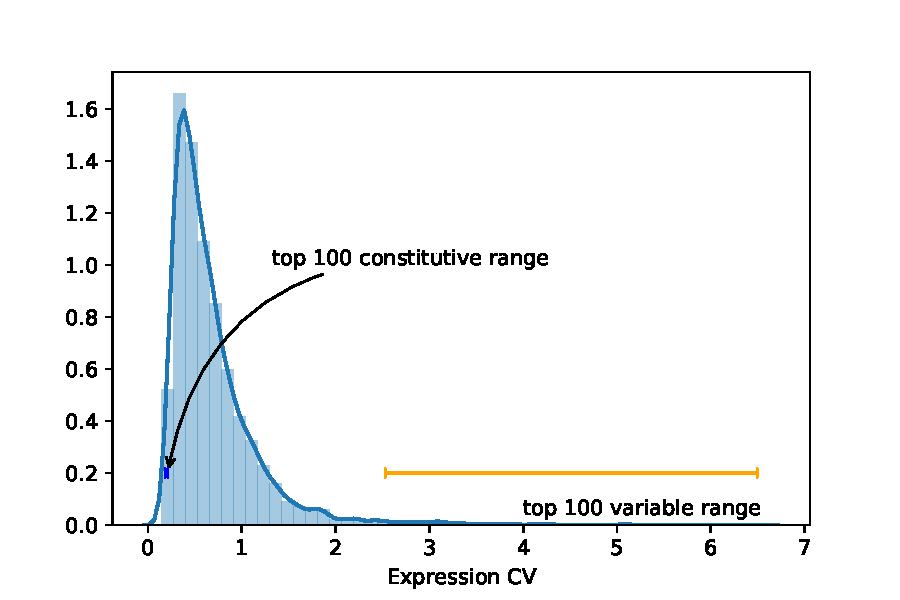
\includegraphics[width=0.70\columnwidth]{genes/czechowski_co-oefficient_of_variation_distribution}
%		\caption{
%			\textbf{Coefficient of expression variation (CV) values for \textit{Arabidopsis thaliana} genes after filtering overlapping genes and genes with no significant TFBSs in their promoters.}
%			CV values calculated as in \textcite{czechowskiGenomeWideIdentificationTesting2005}.
%			The CV range of the top 100 constitutive genes with the lowest CVs is annotated with an arrow (blue range marker).
%			The CV range of the top 100 variable genes with the highest CVs is annotated with an orange range marker).			
%			\label{fig:cv-dist-allgenes}
%		}
%	\end{center}
%\end{figure}


\begin{figure}[hbt!]
	\begin{center}
		\capstart
		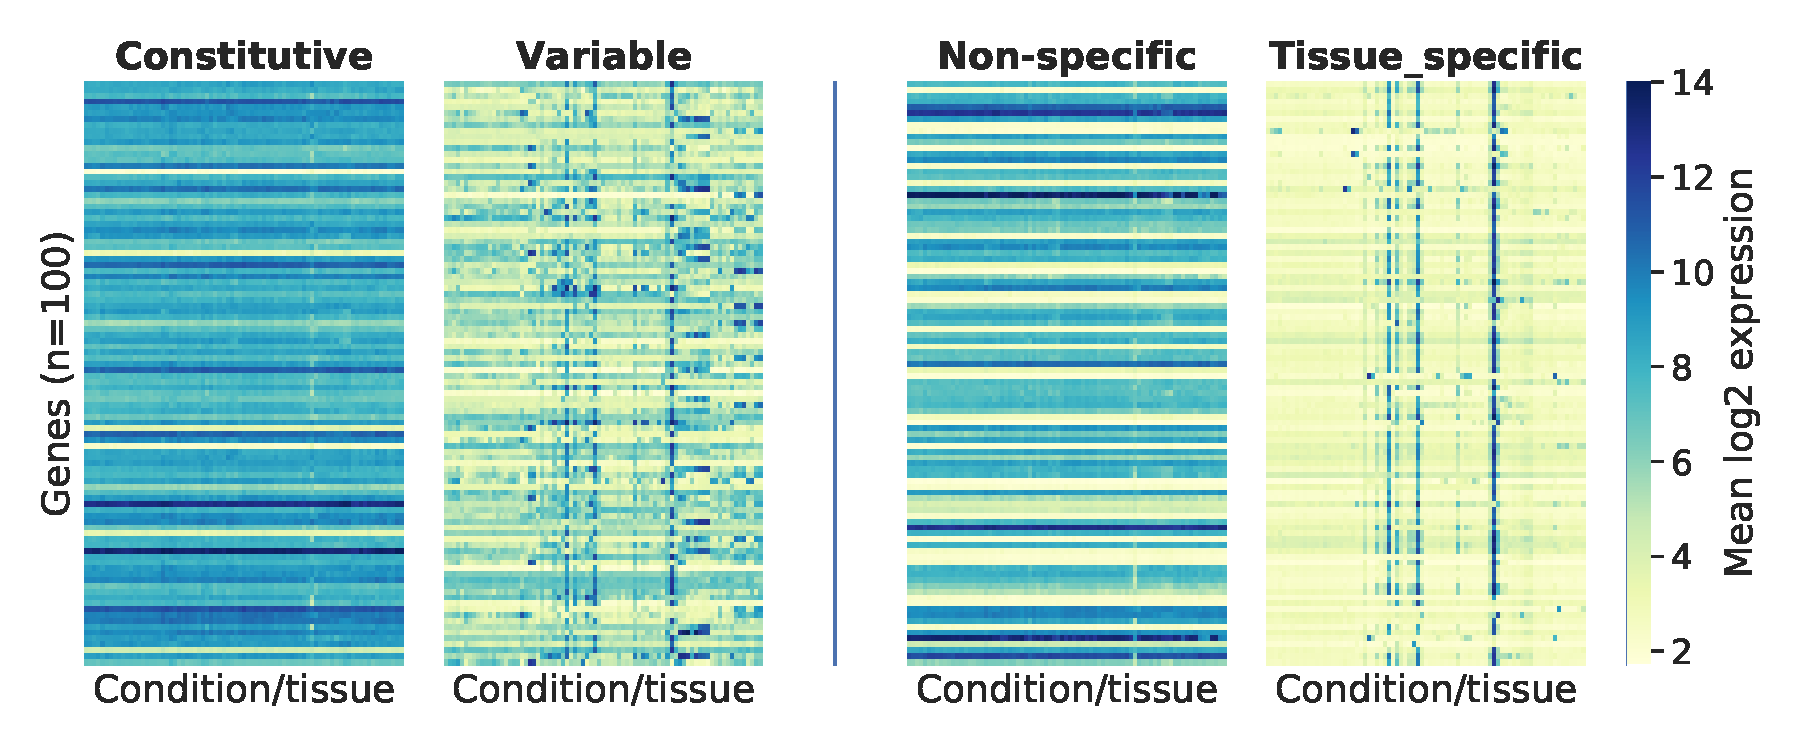
\includegraphics[width=0.80\columnwidth]{genes/gene_group_expression}
		\caption{
			\textbf{Mean log2 expression of constitutive, variable, non\hyp{}specific and tissue\hyp{}specific gene categories in \textit{Arabidopsis thaliana} across 79 different tissues and developmental stages.}
			Constitutive and variable categories chosen using coefficient of variation ranking as in \textcite{czechowskiGenomeWideIdentificationTesting2005}.
			Tissue\hyp{}specific and non\hyp{}specific categories chosen using Tau tissue specificity ranking. \textit{N} = 100.				
			\label{fig:gene_group_expression}
		}
	\end{center}
\end{figure}


A gene ontology (GO) enrichment analysis using Fisher's exact test \autocite{fisherInterpretationContingencyTables1922} and Benjamini/Hochberg FDR correction \autocite{benjaminiControllingFalseDiscovery1995} found four significantly enriched GO terms for the top 300 constitutive genes (\autoref{fig:go-constitutive}), and four significantly enriched GO terms for the top 300 variable genes (\autoref{fig:go-variable}).
In the constitutive group 17 genes were associated with intracellular protein transport, 9 with endocytosis, 4 with receptor mediated endocytosis and 7 genes with the golgi membrane.
Amongst variably expressed genes, 73 were associated with the nucleus, 55 with being extracellular, 32 with the cytosol and 3 with the plastid.
A KEGG gene set enrichment analysis with Benjamini/Hochberg FDR correction found no enriched terms in constitutive or variable groups (\textit{p} \textgreater{} 0.05).

\begin{figure}[hbt!]
	\begin{center}
		\capstart
		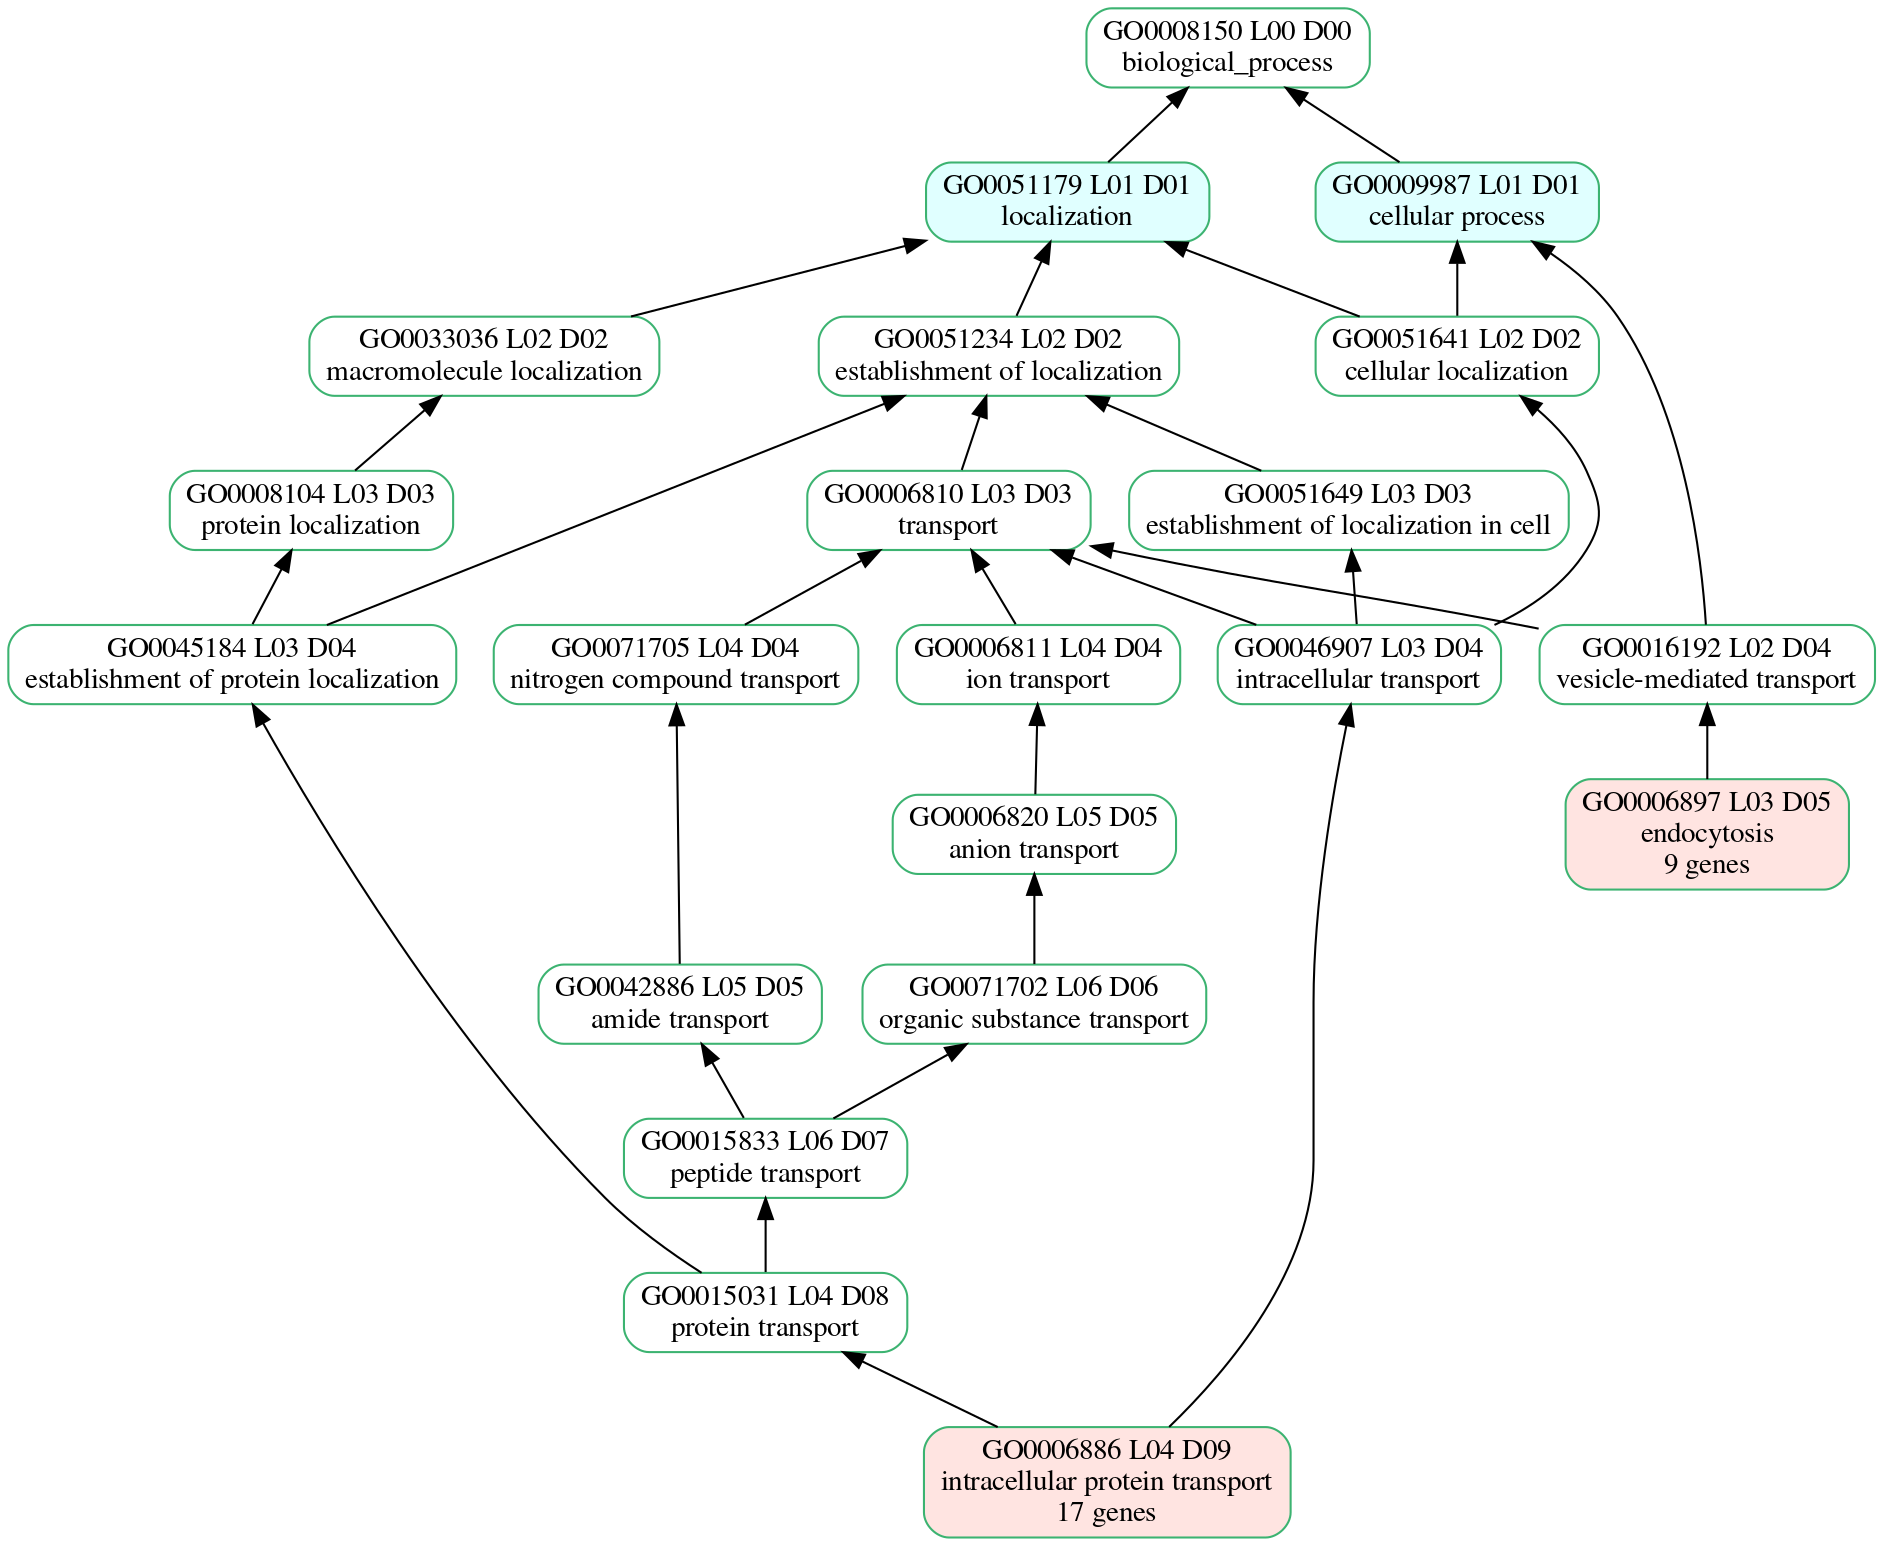
\includegraphics[width=1\columnwidth]{genes/constitutive_Czechowski_sig_enrichment_BP}
		\caption{
			\textbf{Gene ontology lineage plot for the top 300 constitutive \textit{Arabidopsis thaliana} genes.}
			The top 300 constitutive genes were chosen based on coefficient of variation (CV) values as in \textcite{czechowskiGenomeWideIdentificationTesting2005} after filtering overlapping genes and genes with no TFBSs in their promoters.
			Boxes coloured as followed: light red, \textit{p} \textless{} 0.005; yellow, \textit{p} \textless{} 0.05; grey, \textit{p} \textgreater{} 0.05 (non-significant study terms).
			%p < 0.01, light orange
			The gene ontology enrichment analysis was calculated using Fisher's exact test \autocite{fisherInterpretationContingencyTables1922} and Benjamini/Hochberg FDR \autocite{benjaminiControllingFalseDiscovery1995}.
			\label{fig:go-constitutive}
		}
		
	\end{center}
\end{figure}

\begin{figure}[hbt!]
	\begin{center}
		\capstart
		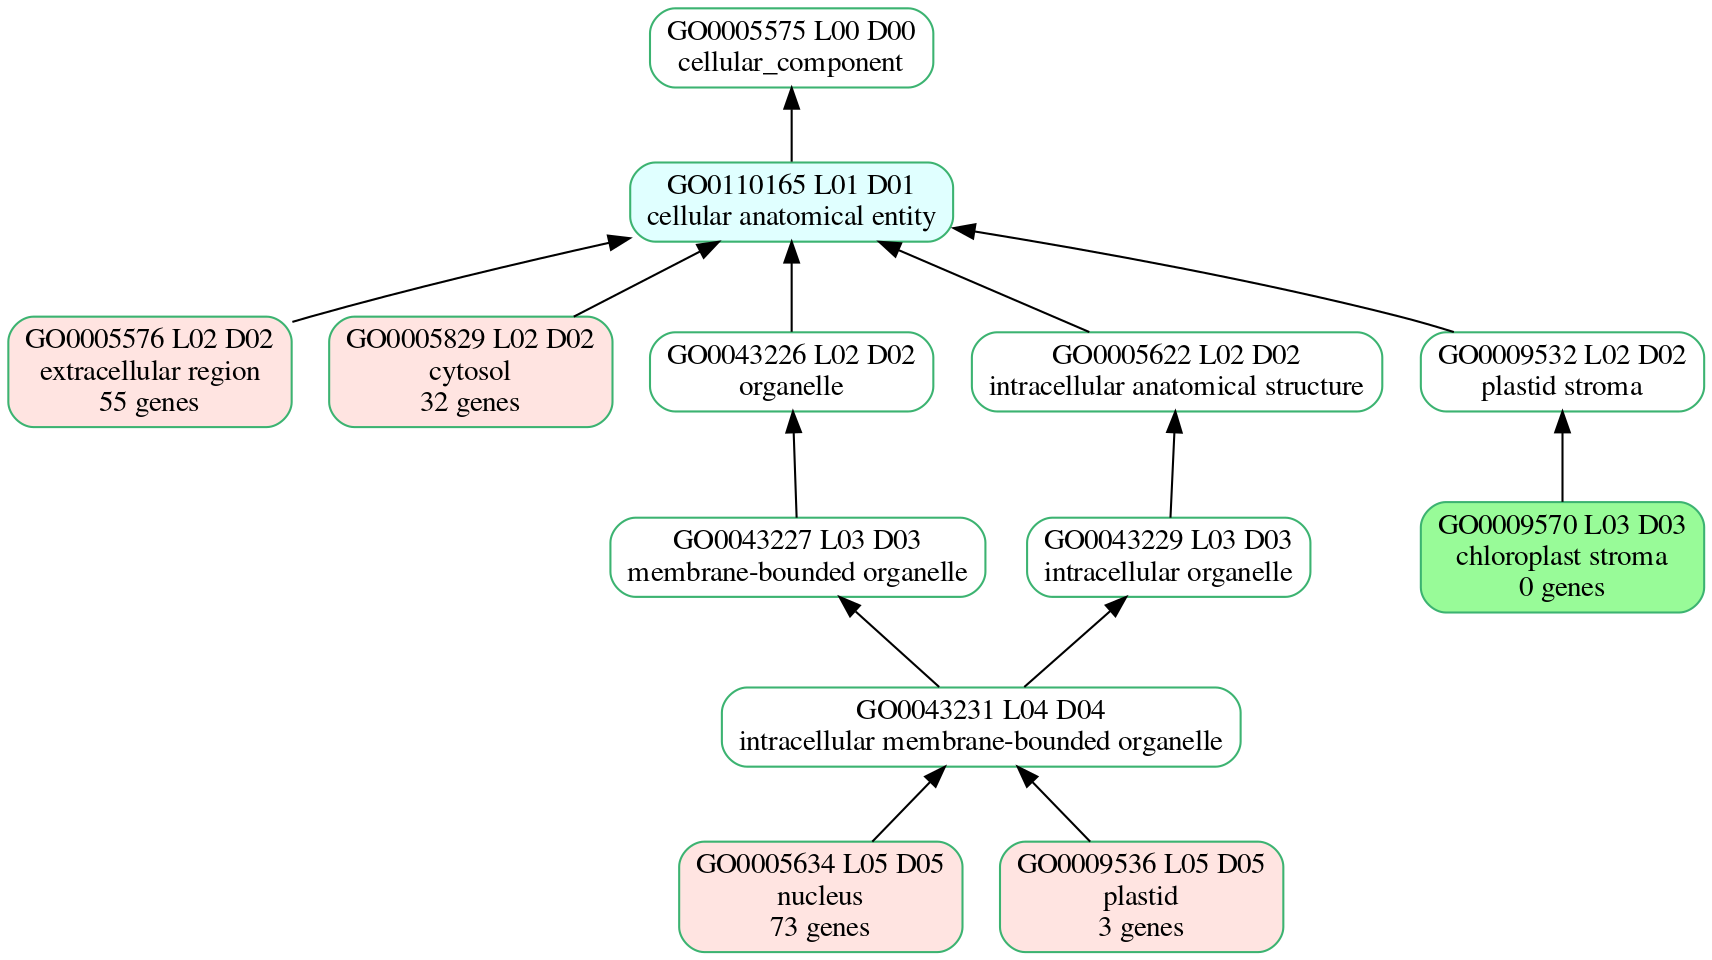
\includegraphics[width=1\columnwidth]{genes/variable_Czechowski_sig_enrichment_CC}
		\caption{
			\textbf{Gene ontology lineage plot for the top 300 variable \textit{Arabidopsis thaliana} genes.}
			The top 300 variable genes were chosen based on coefficient of variation (CV) values as in \textcite{czechowskiGenomeWideIdentificationTesting2005} after filtering overlapping genes and genes with no TFBSs in their promoters.
			Boxes coloured as followed: light red, \textit{p} \textless{} 0.005; grey, \textit{p} \textgreater{} 0.05 (non-significant study terms).
			%p < 0.01, light orange
			The gene ontology enrichment analysis was calculated using Fisher's exact test \autocite{fisherInterpretationContingencyTables1922} and Benjamini/Hochberg FDR correction \autocite{benjaminiControllingFalseDiscovery1995}.
			\label{fig:go-variable}
		}
		
	\end{center}
\end{figure}

\begin{figure}[hbt!]
	\begin{center}
		\capstart
		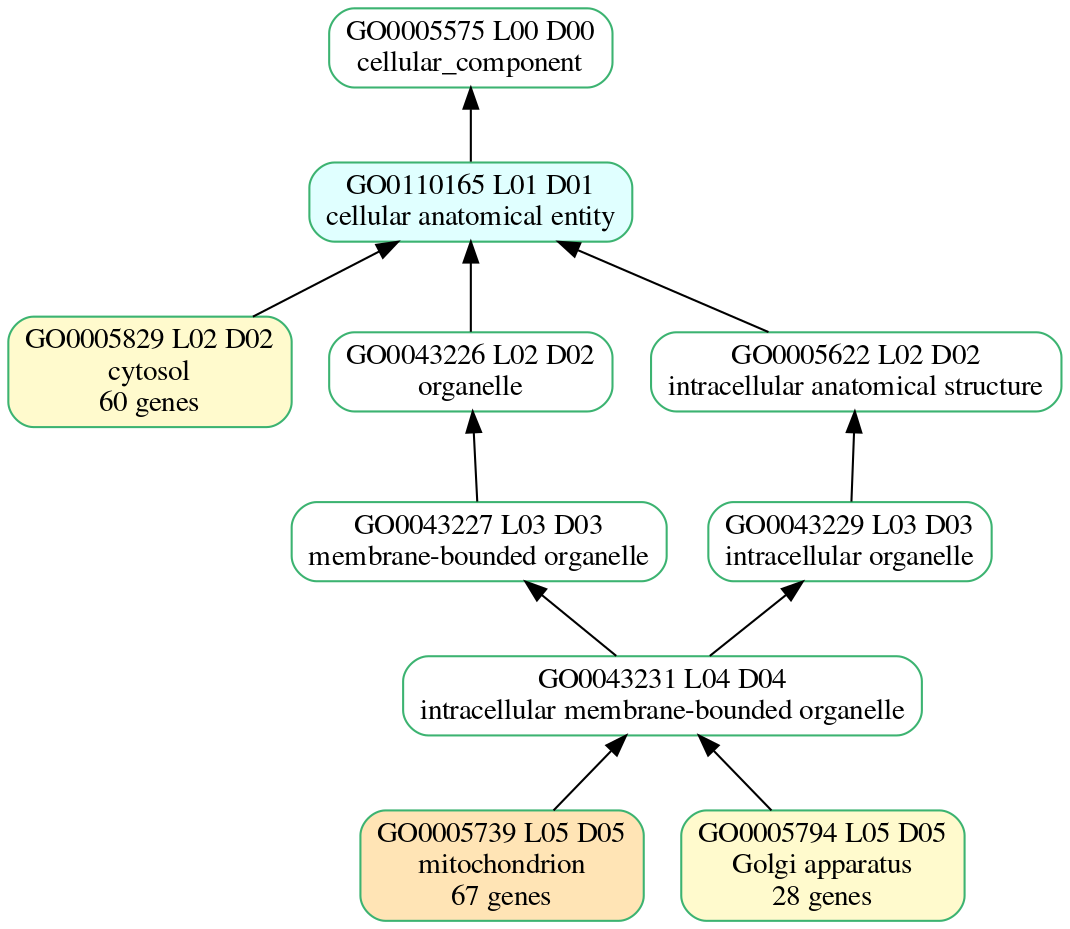
\includegraphics[width=1\columnwidth]{genes/non-specific_Schmid_sig_enrichment_CC}
		\caption{
			\textbf{Gene ontology lineage plot for the top 300 non\hyp{}specific \textit{Arabidopsis thaliana} genes.}
			The top 300 non\hyp{}specific were chosen based on tau tissue\hyp{}specificty values after filtering overlapping genes and genes with no TFBSs in their promoters.
			Boxes coloured as followed: light red, \textit{p} \textless{} 0.005; grey, \textit{p} \textgreater{} 0.05 (non-significant study terms).
			%p < 0.01, light orange
			The gene ontology enrichment analysis was calculated using Fisher's exact test \autocite{fisherInterpretationContingencyTables1922} and Benjamini/Hochberg FDR correction \autocite{benjaminiControllingFalseDiscovery1995}.
			\label{fig:go-variable}
		}
		
	\end{center}
\end{figure}

\begin{figure}[hbt!]
	\begin{center}
		\capstart
		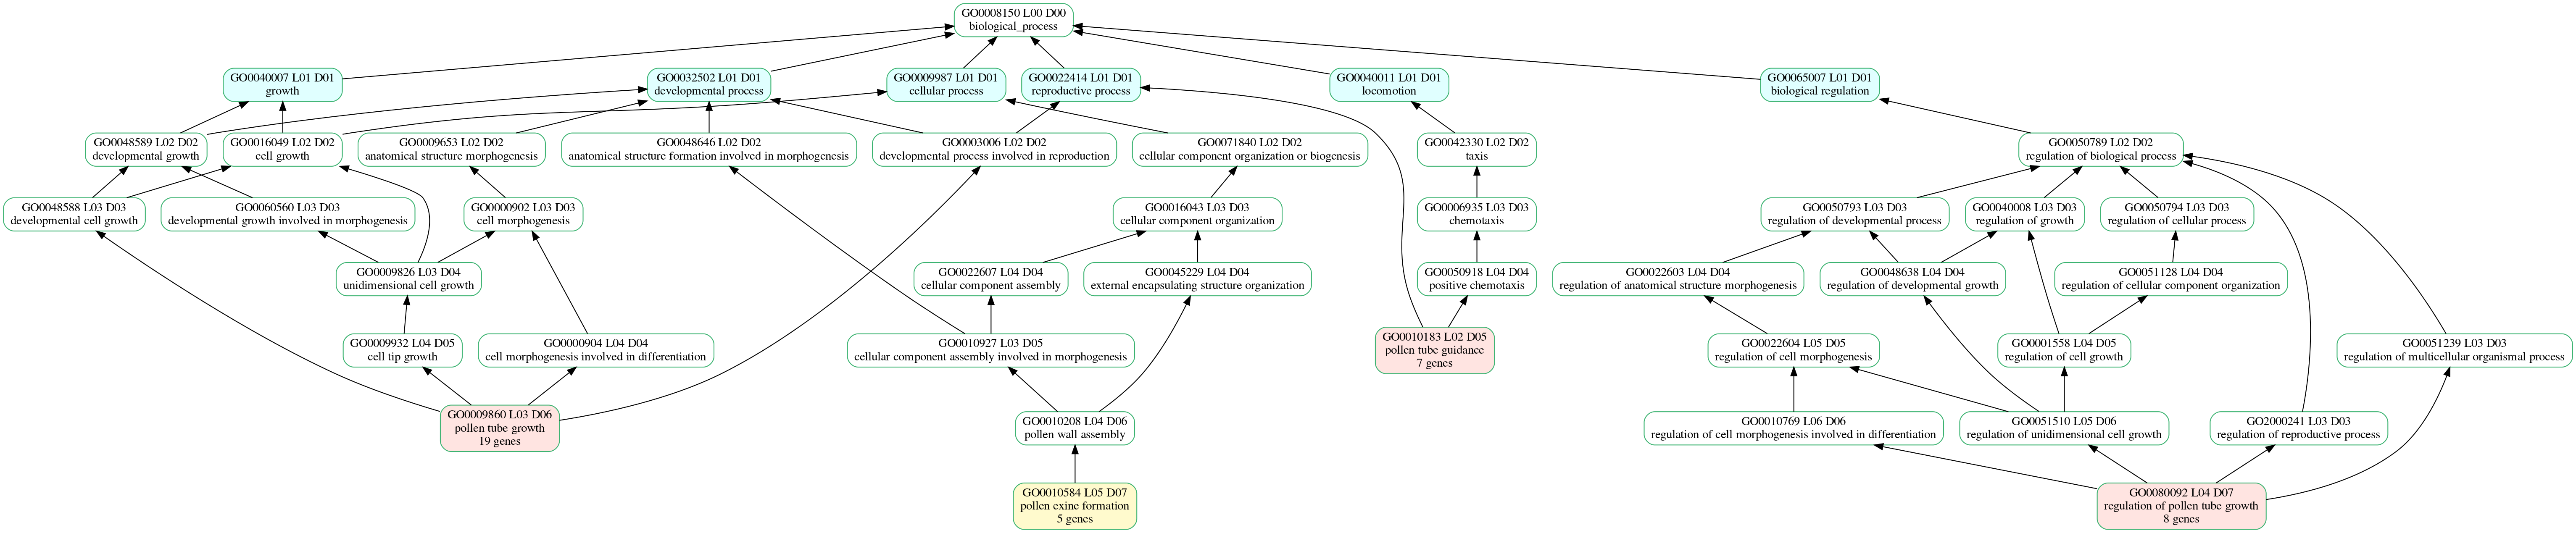
\includegraphics[width=1\columnwidth]{genes/tissue_specific_Schmid_sig_enrichment_BP}
		\caption{
			\textbf{Gene ontology lineage plot for the top 300 tissue\hyp{}specific \textit{Arabidopsis thaliana} genes.}
			The top 300 tissue\hyp{}specific were chosen based on tau tissue\hyp{}specificity values after filtering overlapping genes and genes with no TFBSs in their promoters.
			Boxes coloured as followed: light red, \textit{p} \textless{} 0.005; grey, \textit{p} \textgreater{} 0.05 (non-significant study terms).
			%p < 0.01, light orange
			The gene ontology enrichment analysis was calculated using Fisher's exact test \autocite{fisherInterpretationContingencyTables1922} and Benjamini/Hochberg FDR correction \autocite{benjaminiControllingFalseDiscovery1995}.
			\label{fig:go-variable}
		}
		
	\end{center}
\end{figure}



\subsection{Open chromatin}
CRMs from the four gene sets were overlapped with ATAC-seq data \autocite{potterCytokininModulatesContextdependent2018}. This allowed the chromatin accessibility to be described.

Variable CRMs had a significantly lower percentage of nucleotides covered by open chromatin (\SI{35.0}{\percent}) than constitutive (\SI{54.1}{\percent}) or control (\SI{65.3}{\percent}) CRMs (\autoref{fig:chromatin-coverage}A). Tissue\hyp{}specific CRMs had a significantly lower percentage of nucleotides covered by open chromatin (\SI{20.4}{\percent}) than non\hyp{}specific (\SI{46.9}{\percent}) or control (\SI{65.3}{\percent}) CRMs (\autoref{fig:chromatin-coverage}A)

\begin{figure}[hbt!]
	\begin{center}
		\capstart
		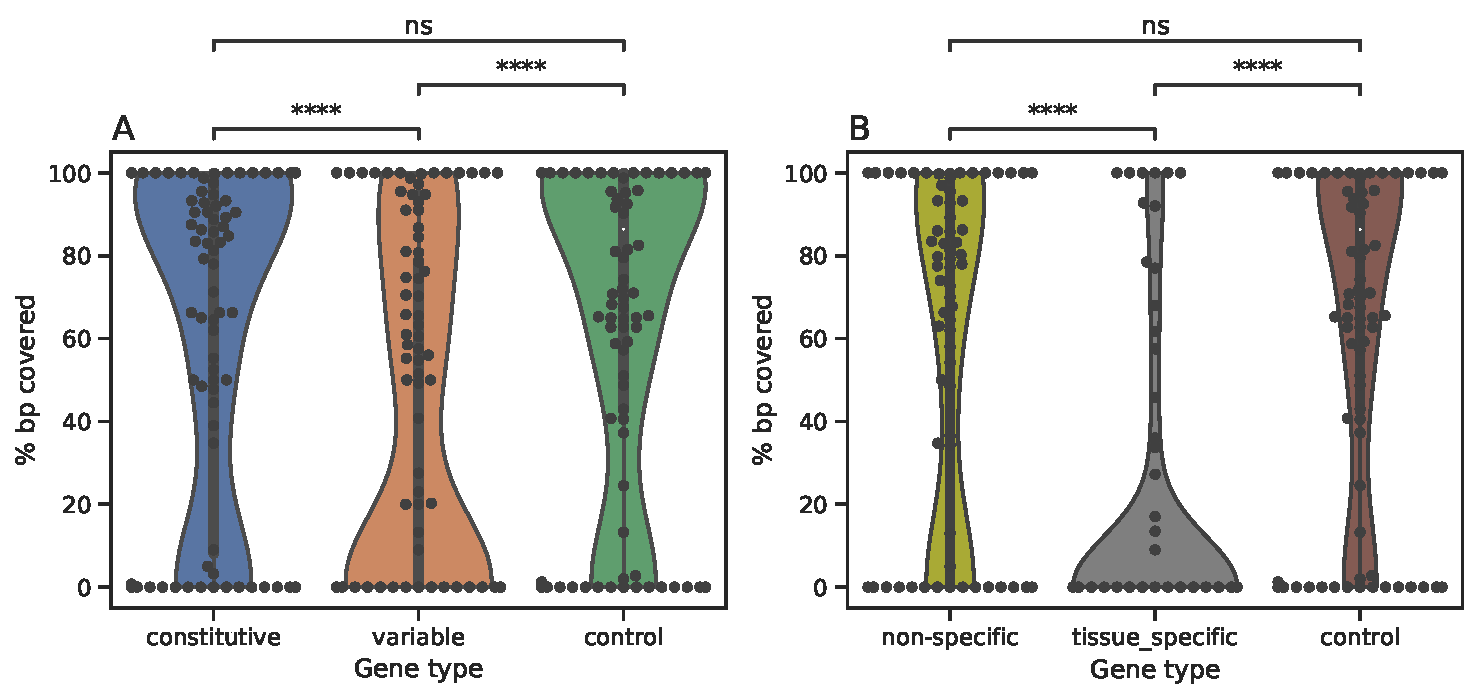
\includegraphics[width=1\columnwidth]{openchromatin/chromatin_coverage_violin}
		\caption{
			\textbf{Percentage open chromatin coverage of 100 constitutive (blue), 100 variable (orange) and 100 control (green) Arabidopsis \textit{cis}\hyp{}regulatory modules (CRMs).}
			Promoters were extracted 1000 bp upstream of the annotated Araport 11 \autocite{chengAraport11CompleteReannotation2017} TSS or until the nearest gene.
			5UTRs were extended downstream of the TSS to the closest coding region.
			Box plots have box boundaries that represent 25th, 50th (median) and 75th percentiles; whiskers are drawn up to the largest or smallest observed point that falls within 1.5 times the interquartile range.
			Significance was calculated using Kruskal\hyp{}Wallis and Dunn's posthocs with Bonferroni correction.
			***, \textit{P} \textless{} 0.001. ****,\textit{P} \textless{} 0.0001. ns, not significant.
			\label{fig:chromatin-coverage}
		}
	\end{center}
\end{figure}
A sliding window analysis revealed that from \textasciitilde{}350 bp to \textasciitilde{}650 bp upstream of the start codon the median open chromatin in constitutive CRMs decreased to zero while variable CRMs had a median percentage open chromatin of 0 (\autoref{fig:openchrom-sliding-window}).

\begin{figure}[!hbt]
	\begin{center}
		\capstart
		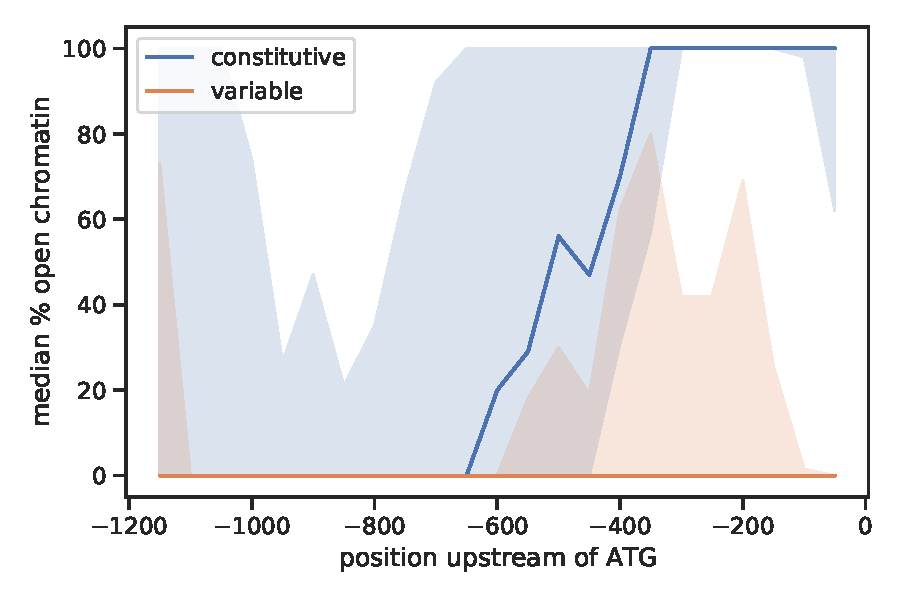
\includegraphics[width=0.8\columnwidth]{openchromatin/Czechowski_genetypenocontrol_percentage_bases_covered_rootshootintersect_chrom_median_sliding_window}
		\caption{
			\textbf{Sliding window analysis of 100 constitutive (blue) and 100 variable (orange) Arabidopsis \textit{cis}\hyp{}regulatory modules (CRMs) upstream of the start codon.}
			Promoters were extracted 1000 bp upstream of the annotated Araport 11 \autocite{chengAraport11CompleteReannotation2017} TSS or until the nearest gene.
			5'UTRs were extended downstream of the TSS to the closest coding region.
			The median proportion of nucleotides falling within open chromatin peaks described by \textcite{potterCytokininModulatesContextdependent2018} was scored for 100 bp windows across selected CRMs.
			The open chromatin peaks used were the intersect of root and shoot peaks derived from the negative control (treated with NaOH) ATAC\hyp{}seq data.
			The windows were overlapping with a 50 bp offset.
			The median value for each bin is displayed here at the central bp of the bin.
			Shading represents 95 confidence intervals estimated using 10000 bootstraps.		
			\label{fig:openchrom-sliding-window}
		}
	\end{center}
\end{figure}

To confirm whether this was a true difference or due to different 5'UTR lengths between constitutive and variable genes, the percentage of root\hyp{}shoot intersect open chromatin of windows was plotted centred around the Araport11 TSS (\autoref{fig:openchrom-sliding-window-araporttss}).
This separated windows located in promoter regions from those in 5'UTRs regions.
The median percentage of open chromatin decreased upstream of the TSS for both constitutive and variable genes, and constitutive genes had a higher percentage open chromatin -100 to + 500 bp around the TSS.



\begin{figure}[!hbt]
	\begin{center}
		\capstart
		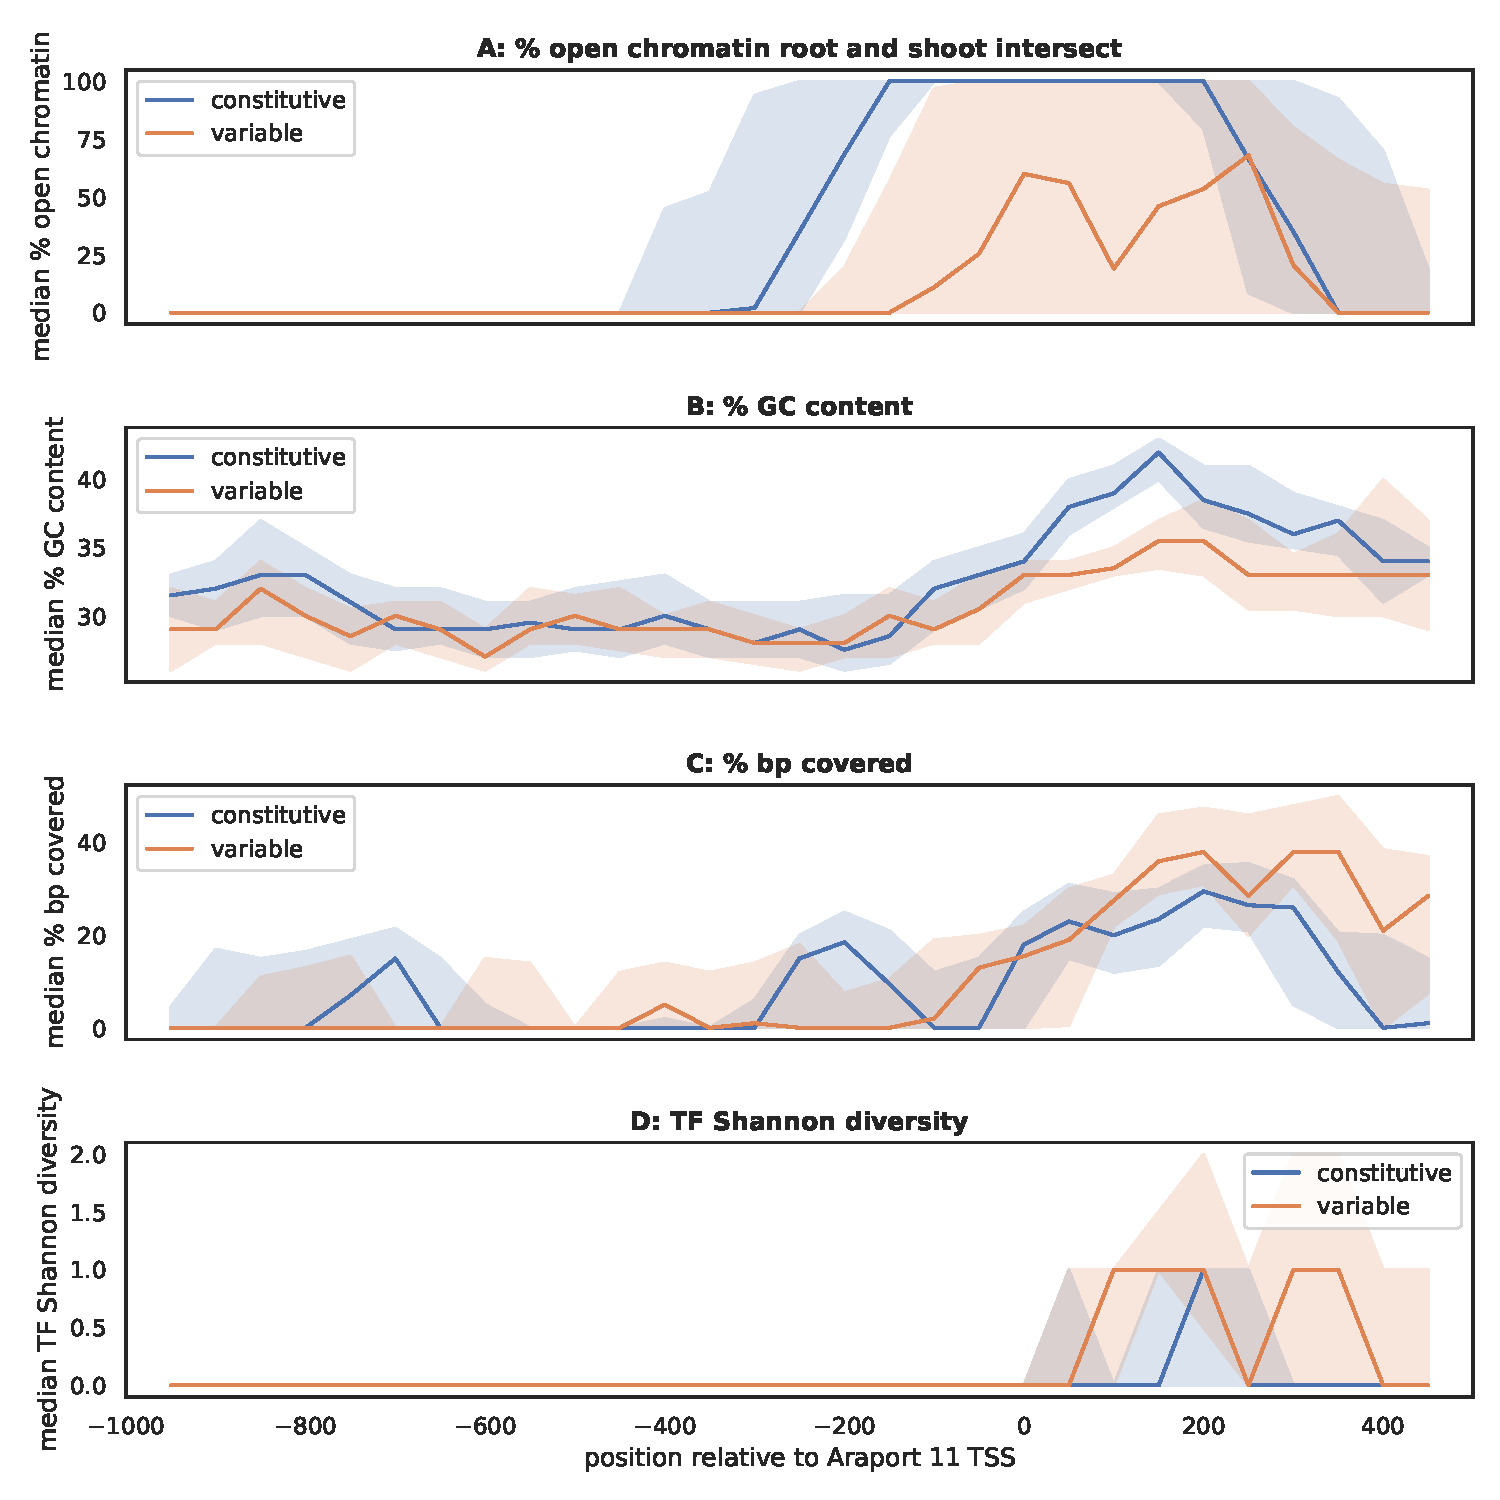
\includegraphics[width=0.8\columnwidth]{openchromatin/Araport11_Czechowski_genetypenocontrol_median_openchromatin_sliding_window}
		\caption{
			\textbf{Sliding window analysis of 100 constitutive (blue) and 100 variable (orange) Arabidopsis \textit{cis}\hyp{}regulatory modules (CRMs) centred around the transcription start site (TSS).}
			Promoters were extracted 1000 bp upstream of the annotated Araport 11 \autocite{chengAraport11CompleteReannotation2017} TSS or until the nearest gene.
			5UTRs were extended downstream of the TSS to the closest coding region.
			TSS is represented by 0 on the x-axis.
			Data points are positioned in the centre of each 100 bp window.
			Windows are offset by 50 bp.
			Shading represents 95 confidence intervals estimated using 10000 bootstraps.
			Median percentage of open chromatin peaks overlapping 100 bp windows. Open chromatin peaks derived from the intersect of root and shoot peaks derived from negative control (treated with NaOH) ATAC\hyp{}seq data by \textcite{potterCytokininModulatesContextdependent2018}.		
			\label{fig:openchrom-sliding-window-araporttss}
		}
	\end{center}
\end{figure}


\subsection{GC content}
%change style to match the start of the previous sections
The hypothesis that constitutive genes have a higher GC content than variable genes was tested.
GC content was not significantly different between variable, constitutive and control promoters (Kruskal\hyp{}Wallis~\textit{H} = 5.8,~\textit{P} \textgreater{} 0.05; \autoref{fig:gc-content-wholeprom}).

\begin{figure}[hbt!]
	\begin{center}
		\capstart
		\includegraphics[width=0.60\columnwidth]{GC_content/wholeprom/Czechowski_GC_content_box}
		\caption{
			\textbf{Percentage GC content of 100 constitutive (blue), 100 variable (orange) and 100 control (green) Arabidopsis \textit{cis}\hyp{}regulatory modules (CRMs).}
			Promoters were extracted 1000 bp upstream of the annotated Araport 11 \autocite{chengAraport11CompleteReannotation2017} TSS or until the nearest gene.
			5UTRs were extended downstream of the TSS to the closest coding region.  Box plots have box boundaries that represent 25th, 50th (median) and 75th percentiles; whiskers are drawn up to the largest or smallest observed point that falls within 1.5 times the interquartile range.
			There was no significant difference in GC content between categories.
			\label{fig:gc-content-wholeprom}
		}
	\end{center}
\end{figure}

A sliding window analysis revealed that percentage GC content looked higher for constitutive genes than variable genes (\autoref{fig:gc-content-sliding-window}.
\begin{figure}[hbt!]
	\begin{center}
		\capstart
		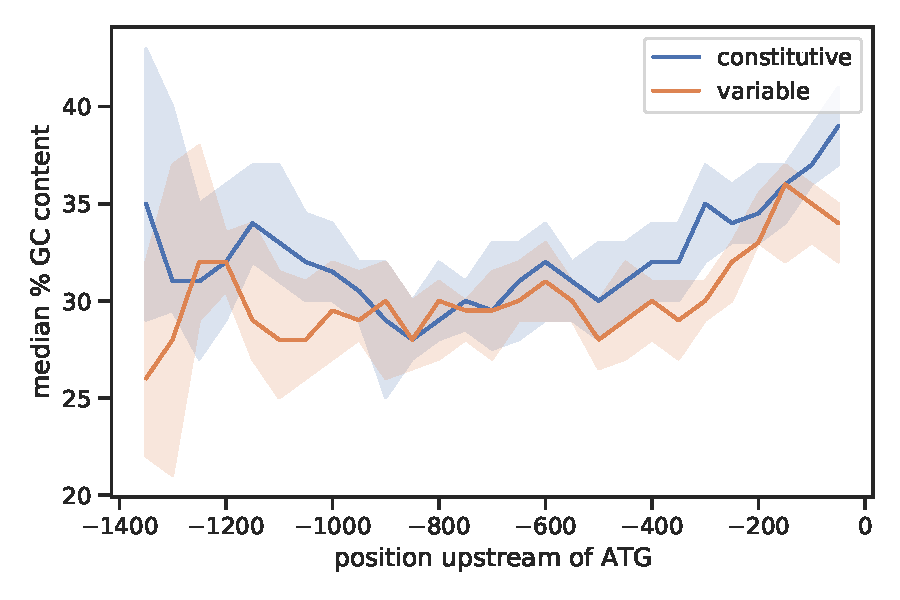
\includegraphics[width=0.8\columnwidth]{GC_content/Czechowski_genetypenocontrol_percentage_GC_content_median_sliding_window}
		\caption{
			\textbf{Sliding window analysis of GC content in 100 constitutive (blue) and 100 variable (orange) Arabidopsis \textit{cis}\hyp{}regulatory modules (CRMs).}
			Promoters were extracted 1000 base pairs (bp) upstream of the annotated Araport 11 \autocite{chengAraport11CompleteReannotation2017} TSS or until the nearest gene.
			5'UTRs were extended downstream of the TSS to the closest coding region.
			The median percentage GC content was scored for 100 bp windows across selected CRMs.
			The windows were overlapping with a 50 bp offset.
			The median value for each bin is displayed here at the central bp of the bin.
			Shading represents 95 confidence intervals estimated using 10000 bootstraps.			
			\label{fig:gc-content-sliding-window}
		}
	\end{center}
\end{figure}

Further analysis in the first 400 bp upstream of the ATG start codon showed that there was a significant difference between promoter types (Kruskal\hyp{}Wallis~\textit{H} = 12.6,~\textit{P} \textless{} 0.01).
Dunn's posthoc tests with Bonferroni correction revealed that within the 400 bp region constitutive promoters had a significantly higher GC content (\SI{35.1}{\percent} ± 5.0) than variable promoters (\SI{33.1}{\percent} ± 4.7; ~\textit{P} \textless{} 0.01) (\autoref{fig:gc-content-400bpprom}).

\begin{figure}[hbt!]
	\begin{center}
		\capstart
		\includegraphics[width=0.60\columnwidth]{GC_content/400bpprom/Czechowski_GC_content_box}
		\caption{
			\textbf{Percentage GC content of 100 constitutive (blue), 100 variable (orange) and 100 control (green) Arabidopsis \textit{cis}\hyp{}regulatory modules (CRMs) in a 400 bp region upstream of the ATG start codon.}
			Box plots have box boundaries that represent 25th, 50th (median) and 75th percentiles; whiskers are drawn up to the largest or smallest observed point that falls within 1.5 times the interquartile range.
			Significance was calculated using Kruskal\hyp{}Wallis and Dunn's posthocs with Bonferroni correction.
			**, \textit{P} \textless{} 0.01. ns, not significant.
			\label{fig:gc-content-400bpprom}
		}
	\end{center}
\end{figure}




\subsection{Transcription factor binding site coverage}
The hypothesis that constitutive genes have a higher TFBS coverage than variable genes was tested.
TFBS coverage was not significantly different between promoter types (Kruskal\hyp{}Wallis~\textit{H} = 5.1,~\textit{P} \textgreater{} 0.05; \autoref{fig:tfbs-coverage-wholeprom}).

\begin{figure}[hbt!]
	\begin{center}
		\capstart
		\includegraphics[width=0.60\columnwidth]{bp_covered/wholeprom/Czechowski_TFBS_coverage_box}
		\caption{
			\textbf{Percentage TFBS coverage of 100 constitutive (blue), 100 variable (orange) and 100 control (green) Arabidopsis \textit{cis}\hyp{}regulatory modules (CRMs).}
			Promoters were extracted 1000 bp upstream of the annotated Araport 11 \autocite{chengAraport11CompleteReannotation2017} TSS or until the nearest gene.
			5UTRs were extended downstream of the TSS to the closest coding region.  Box plots have box boundaries that represent 25th, 50th (median) and 75th percentiles; whiskers are drawn up to the largest or smallest observed point that falls within 1.5 times the interquartile range.
			There was no significant difference in TFBS coverage between categories.
			\label{fig:tfbs-coverage-wholeprom}
		}
	\end{center}
\end{figure}

A sliding window analysis revealed that TFBS coverage was higher in variable promoters than constitutive in the first 400 bp region upstream of the ATG (\autoref{fig:tfbs-coverage-sliding-window}).

 \begin{figure}[hbt!]
	\begin{center}
		\capstart
		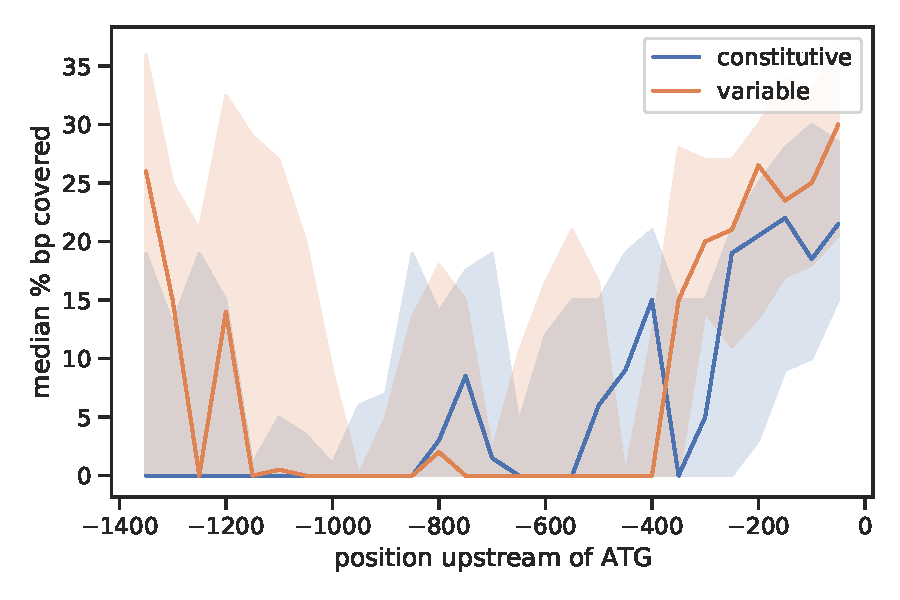
\includegraphics[width=0.8\columnwidth]{bp_covered/Czechowski_genetypenocontrol_percentage_bases_covered_median_sliding_window}
		\caption{
			\textbf{Sliding window analysis of TFBS coverage in 100 constitutive (blue) and 100 variable (orange) Arabidopsis \textit{cis}\hyp{}regulatory modules (CRMs).}
			Promoters were extracted 1000 base pairs (bp) upstream of the annotated Araport 11 \autocite{chengAraport11CompleteReannotation2017} TSS or until the nearest gene.
			5'UTRs were extended downstream of the TSS to the closest coding region.
			The median percentage TFBS coverage was scored for 100 bp windows across selected CRMs.
			The windows were overlapping with a 50 bp offset.
			The median value for each bin is displayed here at the central bp of the bin.
			Shading represents 95 confidence intervals estimated using 10000 bootstraps.
			\label{fig:tfbs-coverage-sliding-window}
		}
	\end{center}
\end{figure}


Further analysis in this 400 bp region revealed a significant difference between promoter types (Kruskal\hyp{}Wallis~\textit{H} = 10.2,~\textit{P} \textless{} 0.01). Dunn's posthocs with Bonferroni correction showed that variable promoters had a significantly higher percentage bp covered (\SI{26.1}{\percent} ± 14.6) than constitutive promoters (\SI{20.0}{\percent} ± 13.7; \textit{P} \textless 0.01; \autoref{fig:tfbs-coverage-400bpprom}).

\begin{figure}[hbt!]
	\begin{center}
		\capstart
		\includegraphics[width=0.60\columnwidth]{bp_covered/400bpprom/Czechowski_TFBS_coverage_box}
		\caption{
			\textbf{Percentage TFBS coverage of 100 constitutive (blue), 100 variable (orange) and 100 control (green) Arabidopsis \textit{cis}\hyp{}regulatory modules (CRMs) in a 400 bp region upstream of the ATG start codon.}
			Box plots have box boundaries that represent 25th, 50th (median) and 75th percentiles; whiskers are drawn up to the largest or smallest observed point that falls within 1.5 times the interquartile range.
			Significance was calculated using Kruskal\hyp{}Wallis and Dunn's posthocs with Bonferroni correction.
			**, \textit{P} \textless{} 0.01. ns, not significant.
			\label{fig:tfbs-coverage-400bpprom}
		}
	\end{center}
\end{figure}

\subsection{TF diversity}
The hypothesis that constitutive genes have a higher diversity of TFs binding them than variable genes was tested.
There was no significant difference in TF (Kruskal\hyp{}Wallis~\textit{H} = 1.1,~\textit{P} \textgreater{} 0.05) or TF family diversity (Kruskal\hyp{}Wallis~\textit{H} = 0.3,~\textit{P} \textgreater{} 0.05) between promoter types \autoref{fig:tf-diversity-wholeprom}).

\begin{figure}[hbt!]
	\begin{center}
		\capstart
		\includegraphics[width=0.6\columnwidth]{TF_diversity/wholeprom/Czechowski_TF_diversity_box_subplots}
		\caption{
			\textbf{Shannon diversity of individual TFs (A) and TF families (B) of 100 constitutive (blue), 100 variable (orange) and 100 control (green) Arabidopsis \textit{cis}\hyp{}regulatory modules (CRMs).}
			Promoters were extracted 1000 bp upstream of the annotated Araport 11 \autocite{chengAraport11CompleteReannotation2017} TSS or until the nearest gene.
			5UTRs were extended downstream of the TSS to the closest coding region.  Box plots have box boundaries that represent 25th, 50th (median) and 75th percentiles; whiskers are drawn up to the largest or smallest observed point that falls within 1.5 times the interquartile range.
			There was no significant difference between categories for either TF Shannon diversity or TF family Shannon diversity.
			\label{fig:tf-diversity-wholeprom}
		}
	\end{center}
\end{figure}

A sliding window analysis revealed that in the constitutive open chromatin region 50-150 bp upstream of the ATG start codon (\autoref{fig:tf-diversity-sliding-window}A) variable promoters looked to have slightly higher Shannon diversity than constitutive promoters (\autoref{fig:tf-diversity-sliding-window}B). Median TF family Shannon diversity did not differ from 0 at any point along the CRM (\autoref{fig:tf-diversity-sliding-window}C).

 \begin{figure}[hbt!]
	\begin{center}
		\capstart
		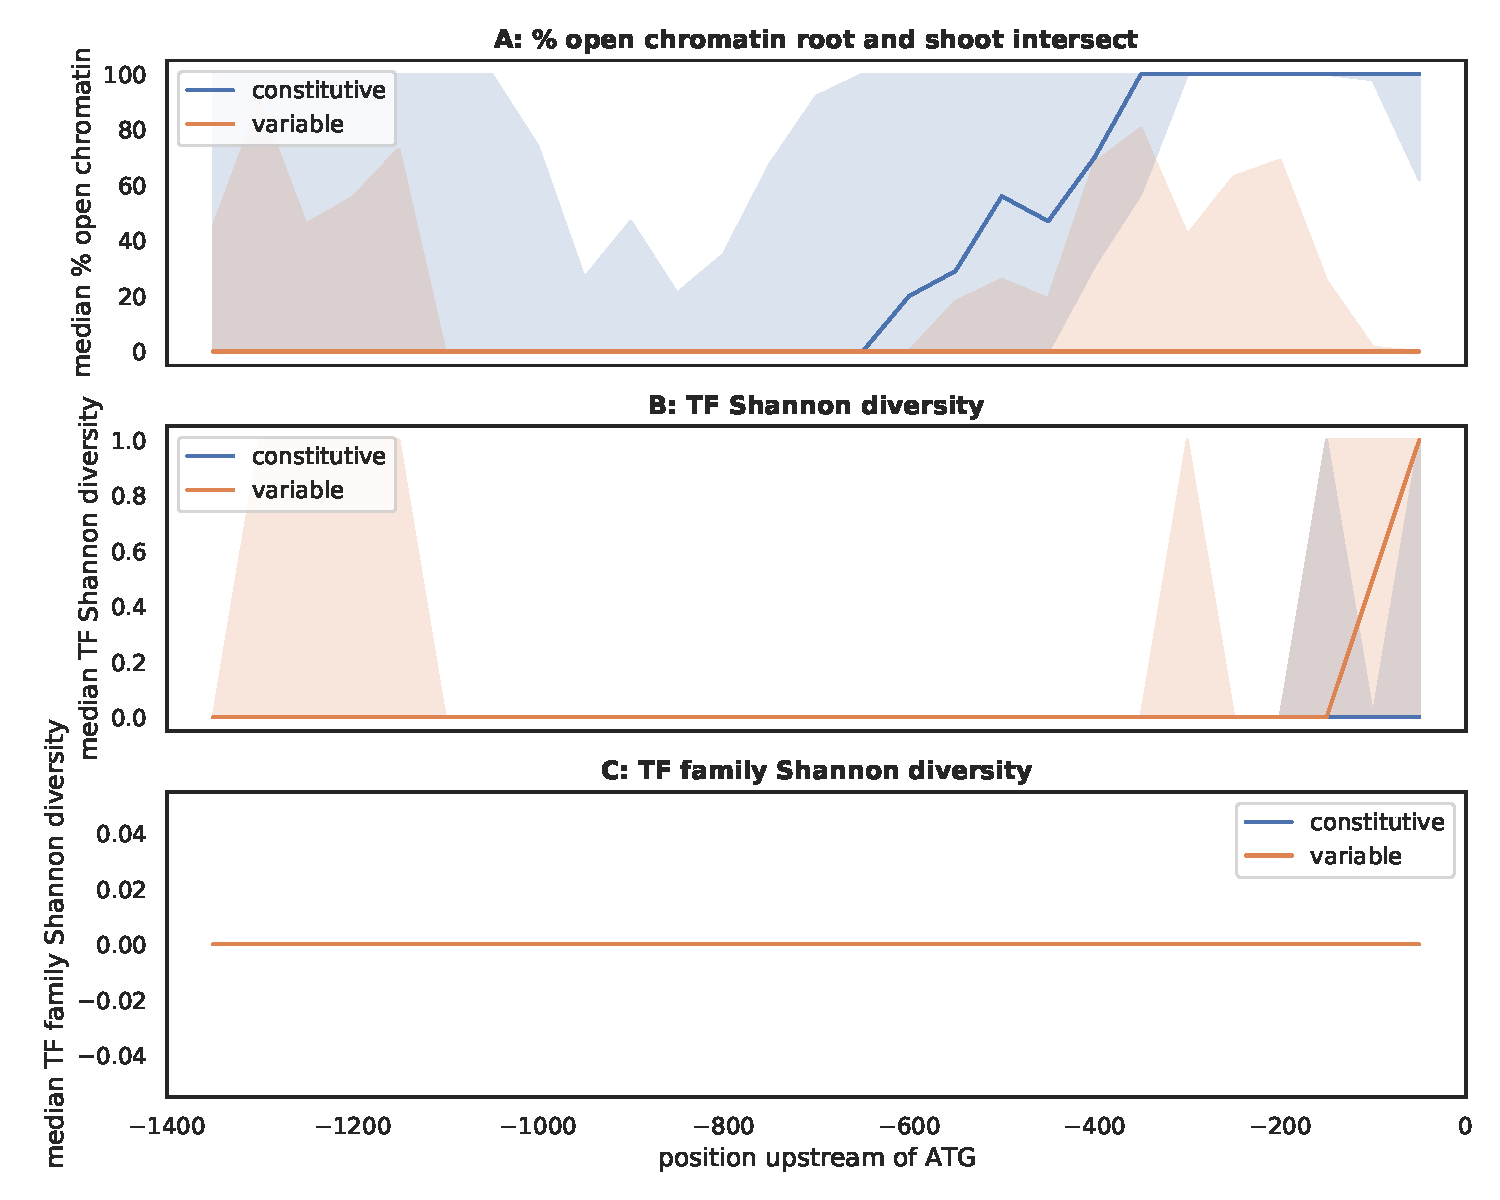
\includegraphics[width=0.8\columnwidth]{TF_diversity/Czechowski_genetypenocontrol_TF_diversity_rw_median_sliding_window_combined}
		\caption{
			\textbf{Sliding window analysis of TF Shannon diversity in 100 constitutive (blue) and 100 variable (orange) Arabidopsis \textit{cis}\hyp{}regulatory modules (CRMs).}
			Promoters were extracted 1000 base pairs (bp) upstream of the annotated Araport 11 \autocite{chengAraport11CompleteReannotation2017} TSS or until the nearest gene.
			5UTRs were extended downstream of the TSS to the closest coding region.
			Data points are positioned in the centre of each 100 bp window.
			Windows are offset by 50 bp.
			Shading represents 95 confidence intervals estimated using 10000 bootstraps.
			A: Median percentage of open chromatin peaks overlapping 100 bp windows. Open chromatin peaks derived from the intersect of root and shoot peaks derived from negative control (treated with NaOH) ATAC\hyp{}seq data by \textcite{potterCytokininModulatesContextdependent2018}.	
			B: Median Shannon diversity of individual TFs in 100 bp windows.
			C: Median Shannon diversity of TF families in 100 bp windows.
			\label{fig:tf-diversity-sliding-window}
		}
	\end{center}
\end{figure}

Further analysis in the 400 bp region upstream of the start codon revealed a significant difference in individual TF diversity between promoter types (Kruskal\hyp{}Wallis~\textit{H} = 6.1,~\textit{P} \textless{} 0.05).
Dunn's posthocs with Bonferroni correction showed that variable promoters had a significantly higher Shannon diversity of individual TFs binding them (\SI{1.6}{\percent} ± 0.7) than constitutive promoters (\SI{1.3}{\percent} ± 0.8; \autoref{fig:tf-diversity-400bpprom}A).
There was no significant difference in the TF family Shannon diversity binding promoters between promoter types (Kruskal\hyp{}Wallis~\textit{H} = 3.3,~\textit{P} \textgreater{} 0.05; \autoref{fig:tf-diversity-400bpprom}B).


\begin{figure}[hbt!]
	\begin{center}
		\capstart
		\includegraphics[width=0.60\columnwidth]{TF_diversity/400bpprom/Czechowski_TF_diversity_box_subplots}
		\caption{
			\textbf{Shannon diversity of individual TFs (A) and TF families (B) of 100 constitutive (blue), 100 variable (orange) and 100 control (green) Arabidopsis \textit{cis}\hyp{}regulatory modules (CRMs) in a 400 bp region upstream of the ATG start codon.}
			Box plots have box boundaries that represent 25th, 50th (median) and 75th percentiles; whiskers are drawn up to the largest or smallest observed point that falls within 1.5 times the interquartile range.
			\label{fig:tf-diversity-400bpprom}
			Significance was calculated using Kruskal\hyp{}Wallis and Dunn's posthocs with Bonferroni correction.
			*, \textit{P} \textless{} 0.05. ns, not significant.
		}
	\end{center}
\end{figure}



\subsection{TATA box enrichment}

Enrichment of 15 bp TATA boxes was compared between constitutive and
variable genes to test the hypothesis that variable genes are enriched in TATA boxes.
Variable promoters were enriched in TATA boxes (total TATA boxes = 53; observed bp=840; expected bp=633; log2fold=0.41;~\textit{P} \textless{} 0.01) compared to the background of all 200 constitutive and variable promoters
(\autoref{fig:tata-enrichment}).
Conversely, constitutive promoters had significantly fewer TATA boxes compared to the background of all 200 constitutive and variable promoters (total TATA boxes = 28; observed bp=440; expected bp=646; log2fold=-0.55;~\textit{P} \textless{} 0.01).

\begin{figure}[!h]
	\begin{center}
		\capstart
		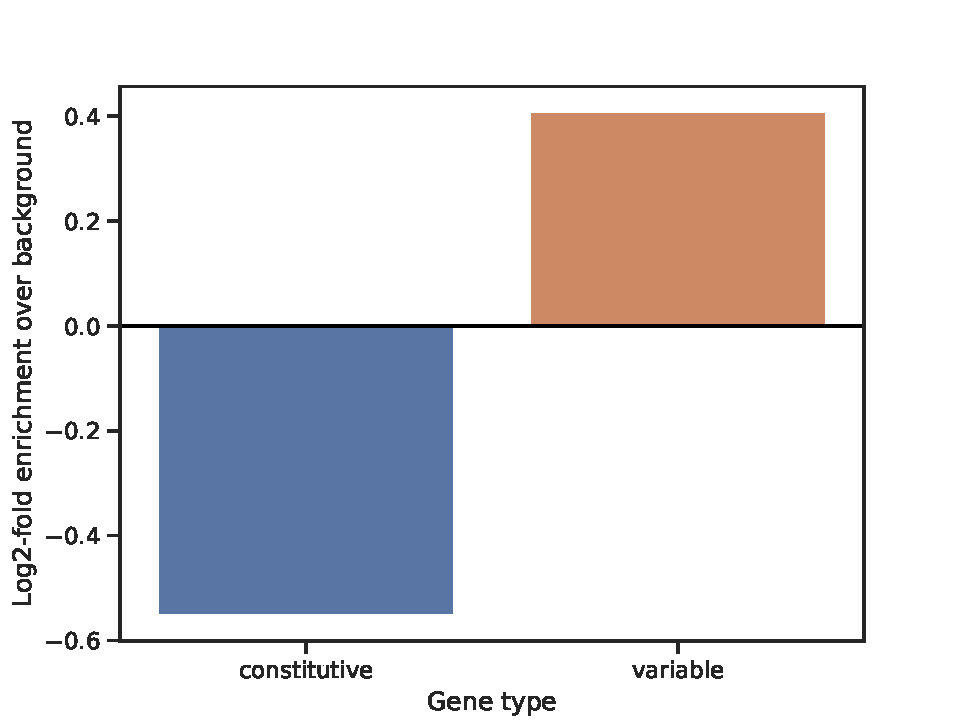
\includegraphics[width=0.70\columnwidth]{log2fold/Czechowski_promoters_5UTR_log2fold}
		\caption{
			\textbf{Log2\hyp{}fold enrichment of 15 bp TATA boxes in 100 variable (blue) and 100 constitutive (orange) Arabidopsis \textit{cis}\hyp{}regulatory modules (CRMs) compared to a background of constitutive and variable promoters combined.}
			Promoters were extracted 1000 bp upstream of the annotated Araport 11 \autocite{chengAraport11CompleteReannotation2017} TSS or until the nearest gene.
			5UTRs were extended downstream of the TSS to the closest coding region.
			TATA box locations within 50 bp upstream of the Eukaryotic Promoter Database (EPD) TSS were downloaded from EPD \autocite{dreosInfluenceRotationalNucleosome2016}.
			 Gat software~\autocite{hegerGATSimulationFramework2013} was used to calculate enrichment.
			\label{fig:tata-enrichment}
		}
	\end{center}
\end{figure}



%TALK ABOUT 5UTR lengths - test if constutive have longer 5'UTR lengths (check for expected  hypothesis first and see if useful comparison or not)
%\begin{figure}[!h]
%	\begin{center}
%		\capstart
%		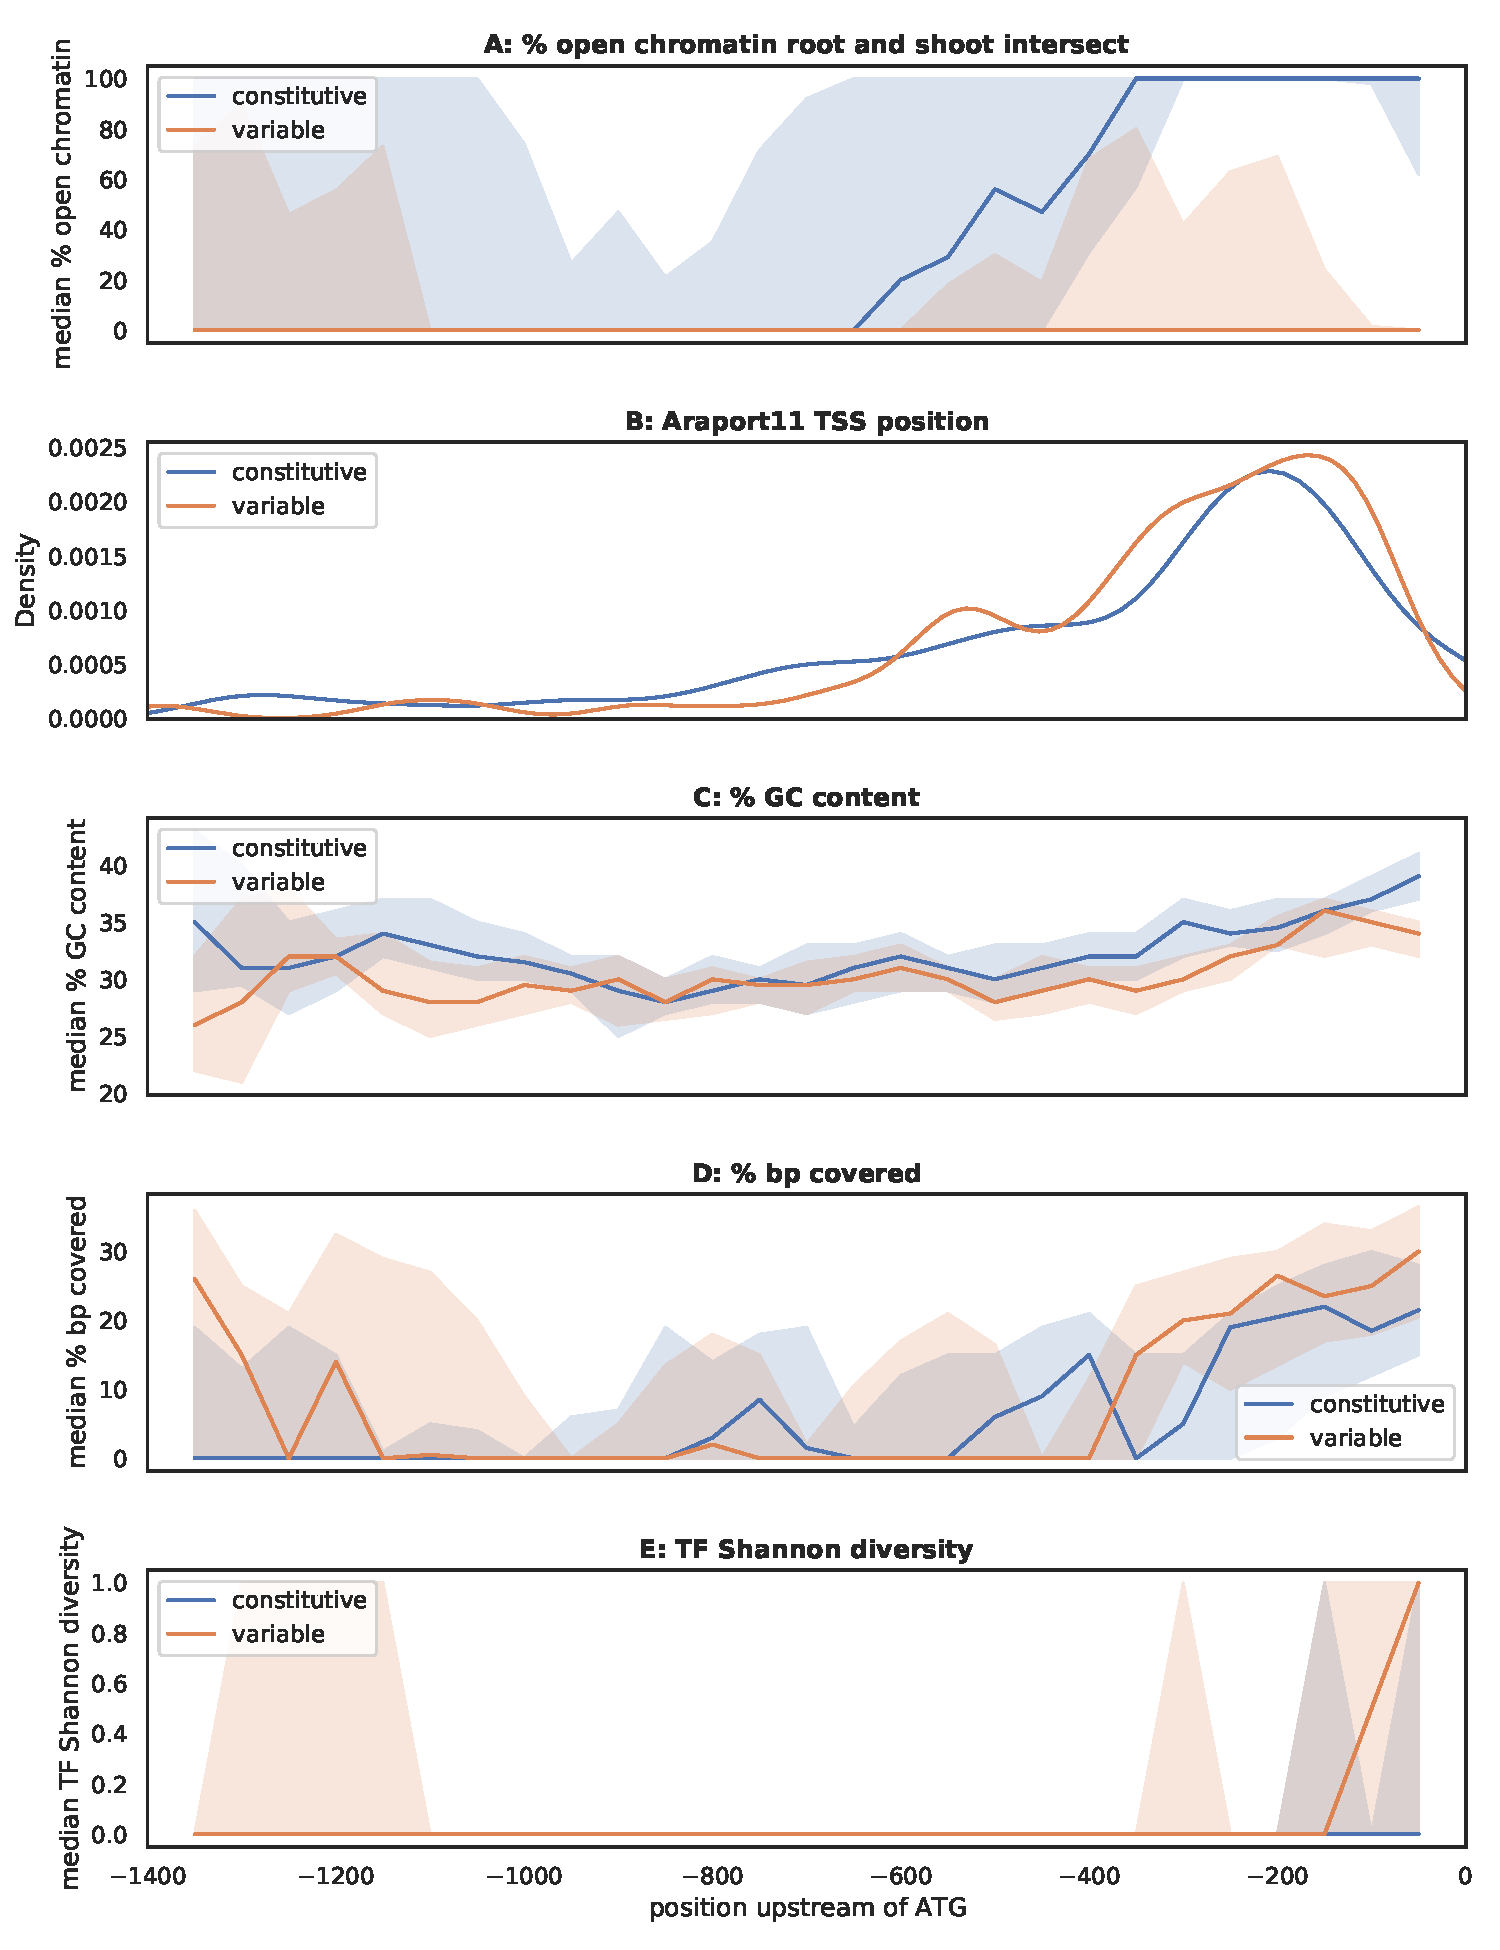
\includegraphics[width=1\columnwidth]{slidingwindow_combined/Czechowski_genetypenocontrol_all_combined_rw_median_sliding_window}
%		\caption{
%			Sliding window analysis of 100 constitutive (blue) and 100 variable (orange) Arabidopsis \textit{cis}\hyp{}regulatory modules (CRMs).
%			Promoters were extracted 1000 base pairs (bp) upstream of the annotated Araport 11 \autocite{chengAraport11CompleteReannotation2017} TSS or until the nearest gene.
%			5UTRs were extended downstream of the TSS to the closest coding region.
%			Data points are positioned in the centre of each 100 bp window.
%			Windows are offset by 50 bp.
%			Shading represents 95 confidence intervals estimated using 10000 bootstraps.
%			A: Median percentage of open chromatin peaks overlapping 100 bp windows. Open chromatin peaks derived from the intersect of root and shoot peaks derived from negative control (treated with NaOH) ATAC\hyp{}seq data by \textcite{potterCytokininModulatesContextdependent2018}.
%			B: Position of Araport11 annotated transcription start site (TSS) upstream of the ATG start codon of the closest coding region.			
%			C: Median percentage GC content in 100 bp windows. N = 95
%			D: Median percentage bp covered by at least one transcription factor binding site.
%			E: Shannon diversity of individual transcription factors binding within each 100 bp window.
%			\label{fig:all-combined-sliding-window}
%		}
%	\end{center}
%\end{figure}

\end{document}


